% ================== Preamble ===================================================

\documentclass[11pt, a4paper, portrait]{scrreprt}
\input{LaTeX-Files/Preamble.tex}
\begin{document}

% ================== Deckblatt ==================================================

\pagenumbering{gobble}
% ================== Frontseite ==================================================
\thispagestyle{empty}
\begin{center}

\vspace*{3cm}

{\Huge\bfseries HSLU Mobile Apps - Android Jetpack Compose - AI First\par}

\vspace{2cm}

{\Large Wirtschaftsprojekt Herbstsemester 2025\par}

\vspace{3cm}

{\Large\textbf{Autoren:} Raphael Eiholzer und Samuel Kurmann\par}

{\Large\textbf{Betreuer:} Jürg Nietlispach\par}

\vfill

{\large Hochschule Luzern – Departement Informatik\par}
{\large Rotkreuz, Schweiz\par}
{\large \today\par}

\end{center}

\newpage
\newpage

\noindent
\fontsize{12}{14}
\textbf{Wirtschaftsprojekt an der Hochschule Luzern -- Informatik} \\ \vspace*{0.6cm}

{\fontsize{11}{12}\selectfont
\noindent
\textbf{Titel: HSLU Mobile Apps - Android Jetpack Compose - AI First} \\ \vspace*{0.2cm}

\noindent
\textbf{Student: Samuel Kurmann} \newline \newline
\textbf{Student: Raphael Eiholzer} \newline \newline
\textbf{Studiengang:} BSc Informatik \newline \newline
\textbf{Jahr: 2025} \newline \newline
\textbf{Betreuungsperson: Jürg Nietlispach} \newline \newline
\textbf{Experte: Martin Vogel} \newline \newline
\textbf{Auftraggeber: Jürg Nietlispach / Departement Informatik} \newline \newline
\textbf{Codierung / Klassifizierung der Arbeit:}\\
$\square$ Öffentlich \quad $\square$ Vertraulich

\vspace*{1cm}

\paragraph*{\textbf{Eidesstattliche Erklärung}}
Ich erkläre hiermit, dass wir die vorliegende Arbeit selbständig und ohne unerlaubte fremde Hilfe angefertigt haben, alle verwendeten Quellen, Literatur und andere Hilfsmittel angegeben haben, wörtlich oder inhaltlich entnommene Stellen als solche kenntlich gemacht haben, das Vertraulichkeitsinteresse des Auftraggebers wahren und die Urheberrechtsbestimmungen der Hochschule Luzern respektieren werden.

\vspace*{1cm}
Ort / Datum, Unterschrift \underline{\hspace*{8cm}} \newline \newline
Ort / Datum, Unterschrift \underline{\hspace*{8cm}} \newline \newline

\textbf{Ausschliesslich bei Abgabe in gedruckter Form:}\\
Eingangsvisum durch das Sekretariat auszufüllen

\vspace*{0.5cm}
Rotkreuz, den \underline{\hspace*{4cm}} \hspace*{1cm} Visum: \underline{\hspace*{4cm}}

\newpage

% ================== Inhalt =====================================================

\pagenumbering{roman}

\chapter*{Abstract / Zusammenfassung oder Management Summary}
\addcontentsline{toc}{chapter}{Abstract}
Im Rahmen des Wirtschaftsprojekts \emph{HSLU Mobile Apps – Android Jetpack Compose – AI First}
wurde eine bestehende Android-Applikation der Hochschule Luzern technisch neu umgesetzt.
Ausgangslage war eine veraltete Android-App auf Basis von XML-Layouts sowie eine moderne
iOS-Applikation, welche als Referenz diente. Ziel des Projekts war es, eine zeitgemässe
Android-Applikation mit Jetpack Compose zu realisieren, die funktional an die iOS-Version
angeglichen ist, aktuelle Android-Technologien nutzt und produktiv im Google Play Store
veröffentlicht werden kann.

Die Umsetzung erfolgte über ein agiles Vorgehen mit zweiwöchigen Sprints. Zu Projektbeginn
wurde gemeinsam mit dem Auftraggeber ein klarer Rahmen definiert, inklusive regelmässiger
Status-Meetings und transparenter Aufgabenverwaltung über GitLab. Die Entwicklung wurde
modular aufgebaut. Gemeinsame,
fachlich unabhängige Komponenten wurden in zentralen \texttt{common}-Modulen umgesetzt,
während einzelne Features wie News, Blog, Mensa, Events oder Raumsuche jeweils als eigene
Module realisiert wurden. Diese Struktur wurde dabei von der bestehenden iOS-Applikation
übernommen, um eine einheitliche Architektur über beide Plattformen hinweg sicherzustellen.

Ein Schwerpunkt des Projekts lag auf dem AI-First-Ansatz.
KI-gestützte Entwicklungswerkzeuge wurden getestet und dann aktiv in den Entwicklungsprozess eingebunden. 
AI wurde unter anderem für Code-Analysen,
Übersetzungen von bestehendem iOS-Code nach Kotlin, Unterstützung bei neuen Features
sowie für das Testing eingesetzt. Die Erfahrungen zeigen, dass AI insbesondere
bei klar abgegrenzten Aufgaben und gut formulierten Prompts eine deutliche Zeitersparnis
ermöglicht, gleichzeitig aber weiterhin fundierte Programmierkenntnisse notwendig bleiben.

Als Resultat steht eine moderne, modular aufgebaute Android-Applikation auf Basis von
Jetpack Compose zur Verfügung, die Multi-Tenant-fähig ist, aktuelle Android-SDKs
unterstützt und automatisiert über CI/CD und Fastlane ausgeliefert werden kann.
Ergänzend dazu wurden alle Projektartefakte wie Dokumentation, Risikoanalyse,
Sprint-Backlogs, Statusberichte und Protokolle vollständig erstellt, sodass eine
Weiterentwicklung des Projekts problemlos möglich ist. \newpage

\newpage
\tableofcontents
\newpage

% ================== Hauptteil ==================================================

\pagenumbering{arabic}

\chapter{Problem, Fragestellung, Vision}
Beschreibe das Problem, die Zielsetzung und die übergeordnete Vision des Projekts.

\section{Ausgangslage und Problemstellung}\vspace{-1.5em}

Die Hochschule Luzern betreibt für die Departemente Informatik sowie Technik \& Architektur eigene mobile
Applikationen auf den Plattformen iOS und Android. Während die iOS-Applikation in den vergangenen
Semestern weiterentwickelt wurde,
befindet sich die Android-Version aktuell in einem teilweise veralteten Zustand.

Auf Android existiert einerseits eine veröffentlichte Applikation auf Basis klassischer XML-Layouts, welche
weder an das aktuelle Backend-API angebunden ist noch alle Features der iOS-Version enthält. 
Andererseits liegt eine nicht veröffentlichte Jetpack-Compose-Applikation vor, die zwar
bereits auf einem deklarativen UI-Ansatz basiert, jedoch ebenfalls nicht mehr dem aktuellen Stand der
Technik entspricht und funktional hinter der iOS-Version zurückbleibt.

Diese Situation führt dazu, dass der Entwicklungsstand der Android-Applikationen weit hinter der iOS-Applikationen zurückliegt. 
Eine konsistente App-Landschaft über beide Plattformen hinweg ist nicht gegeben. Gleichzeitig besteht der
Anspruch, neue Features, die auf iOS bereits umgesetzt wurden, auch auf Android bereitzustellen.
Vor diesem Hintergrund ergibt sich das Bedürfnis, die bestehende Android-Jetpack-Compose-
Applikation grundlegend zu modernisieren und funktional an die iOS-Applikationen anzugleichen. 

\section{Ziel der Arbeit und erwartete Resultate}\vspace{-1.5em}

Ziel dieses Projekts ist die Umsetzung einer modernen
Android-Applikation auf Basis von Jetpack Compose, welche an die bestehende
iOS-App der Hochschule Luzern angeglichen ist. Die Applikation soll aber auch Android-
Technologien und Architekturkonzepte nutzen, wartbar und erweiterbar aufgebaut sein,
um dann produktiv über den Google Play Store veröffentlicht werden zu können.

Die Umsetzung soll als modulare Single-Codebase mit Unterstützung für mehrere
Features und Mandanten (Multi-Tenant) erfolgen. Die Architektur soll sich
an der bestehenden iOS-Applikation orientieren, um eine möglichst einheitliche
Plattformstruktur zu erreichen, damit künftige Arbeiten auf beiden Plattformen einfacher zu erledigen sind.

Ein weiterer zentraler Aspekt der Arbeit soll der Einsatz eines AI-First-Ansatzes sein. Ziel ist es,
verschiedene KI-gestützte Entwicklungswerkzeuge im Kontext der mobilen
App-Entwicklung zu evaluieren und deren Einsatzmöglichkeiten, Grenzen und Mehrwerte
praktisch zu untersuchen. Die gewonnenen Erkenntnisse sollen dokumentiert und
reflektiert werden. (Die vollständige Aufgabenstellung ist zu finden im Anhang: ~\ref{sec:aufgabenstellung}).

Die erwarteten Resultate lassen sich wie folgt zusammenfassen:

\begin{itemize}
    \item \textbf{App-Artefakte:}
    \begin{itemize}
        \item Eine produktiv einsetzbare Android-Applikation auf Basis von Jetpack Compose
        \item Umsetzung und Integration der fehlenden bzw. neu aufgebauten Features
        \item Anbindung an das aktuelle Backend-API
        \item Unterstützung aktueller Android-SDKs und Geräte
        \item Automatisierter Build- und Release-Prozess mittels GitLab CI/CD und Fastlane
    \end{itemize}

    \item \textbf{Projektmanagement-Artefakte:}
    \begin{itemize}
        \item Sprint-basierte Planung und Umsetzung mit dokumentierten Issues und Epics
        \item Regelmässige Statusberichte und Sitzungsprotokolle
        \item Fortlaufende Risikoanalyse und Meilensteinübersicht
    \end{itemize}

    \item \textbf{Dokumentation und Evaluation:}
    \begin{itemize}
        \item Projektdokumentation gemäss HSLU-Standards
        \item Evaluation und Reflexion des AI-First-Ansatzes im Entwicklungsprozess
        \item Zwischen- und Schlusspräsentation der Projektergebnisse
    \end{itemize}
\end{itemize}

\chapter{Stand der Praxis}
In der aktuellen Ausgangslage existieren drei unterschiedliche mobile Applikationen, die sich sowohl hinsichtlich ihres technologischen Stands als auch ihres Funktionsumfangs 
deutlich voneinander unterscheiden. Diese Situation erfordert eine klare Einordnung der bestehenden Lösungen sowie eine strategische Ausrichtung für die Weiterentwicklung der 
Android-Plattform.

Zum einen gibt es eine veröffentlichte Android-Applikation, die auf klassischen XML-Layouts basiert. Diese Anwendung ist bereits seit längerer Zeit im Einsatz, nutzt jedoch weder 
alle verfügbaren Funktionen noch moderne Android-Entwicklungskonzepte. Wichtige aktuelle Technologien und Best Practices, wie sie heute im Android-Ökosystem etabliert sind, wurden 
in dieser App nicht oder nur unzureichend berücksichtigt. Dadurch entspricht sie nicht mehr dem aktuellen Stand der Technik und weist sowohl in Bezug auf 
Wartbarkeit als auch auf Benutzererlebnis klare Defizite auf. Erweiterungen oder Anpassungen sind dadurch aufwendiger und weniger nachhaltig umsetzbar.

Parallel dazu existiert eine iOS-Applikation, die sich auf einem aktuellen technischen Stand befindet und ebenfalls bereits veröffentlicht ist. Diese App nutzt moderne 
Entwicklungsansätze und implementiert die gewünschten Funktionen vollständig und zeitgemäss. Sie stellt damit eine stabile, ausgereifte und zukunftsfähige Lösung dar. 
Aufgrund ihres aktuellen Zustands und der vollständigen Feature-Abdeckung dient diese iOS-Applikation als fachliche und funktionale Referenz. An ihr kann und soll sich 
die Weiterentwicklung der Android-Anwendungen orientieren, insbesondere im Hinblick auf Funktionsumfang, Benutzerführung und technisches Design.

Als dritte Variante liegt zudem eine Android-Applikation auf Basis von Jetpack Compose vor. Diese App ist aktuell nicht veröffentlicht und ebenfalls veraltet. 
Obwohl Jetpack Compose grundsätzlich ein modernes UI-Framework darstellt, wurde die Anwendung seit längerer Zeit nicht mehr aktualisiert und nutzt weder die aktuellen 
Möglichkeiten von Compose noch moderne Architektur- und State-Management-Konzepte. Funktional und technisch kann sie daher nicht als zeitgemäss betrachtet werden. 
Gleichzeitig bietet sie jedoch eine gute Grundlage für eine moderne Android-Neuentwicklung, da sie bereits auf einem deklarativen UI-Ansatz basiert.

Ziel ist es nun, diese Android-Jetpack-Compose-Applikation gezielt zu modernisieren und weiterzuentwickeln. Dabei soll sie technologisch auf den neuesten Stand 
gebracht und funktional an die bestehende iOS-Applikation angeglichen werden. Die iOS-App dient hierbei als Referenz für Features, Benutzererlebnis und funktionale Vollständigkeit. 
Durch diese Ausrichtung kann sichergestellt werden, dass künftig eine konsistente und moderne App-Landschaft auf beiden Plattformen existiert, die sowohl den aktuellen technischen 
Standards entspricht als auch eine einheitliche Nutzererfahrung bietet.


\chapter{Ideen und Konzepte}
\section{Konzept zur Übernahme der iOS-Applikation auf Android}

Die Android-Applikation soll auf Basis von Jetpack Compose funktional auf
denselben Stand gebracht werden wie die aktuelle Dev-Version der
iOS-Applikation. Die iOS-App dient dabei aus unserer Sicht als vollständige
Referenz, sowohl in Bezug auf den Funktionsumfang als auch auf den
grundsätzlichen Aufbau der Applikation. Ziel ist es, dass beide Plattformen
möglichst ähnlich strukturiert sind, um zukünftige Arbeiten zu vereinfachen
und den Einstieg für neue Entwicklerinnen und Entwickler zu erleichtern.

Eine vollständige 1:1-Übernahme ist dabei nicht in allen Bereichen möglich,
da sich iOS und Android sowie die Programmiersprachen Swift und Kotlin in
einigen Aspekten unterscheiden. Dennoch sollen das grundlegende Vorgehen,
die Projektstruktur sowie die Benennung von Modulen und Komponenten so weit
wie möglich angeglichen werden. Wie bereits bei der iOS-Applikation soll
auch die Android-App klar in \texttt{Common}-Komponenten und einzelne
\texttt{Feature}-Module unterteilt werden, damit fachlich unabhängige Logik
zentral wiederverwendet werden kann.

\vspace{0.5em}
\begin{figure}[H]
    \centering
    \includegraphics[width=0.43\textwidth]{Fotos/ios-projektstruktur.png}
    \caption{iOS-Projektstruktur in XCode}
    \label{fig:iosprojektstrukur}
\end{figure}

\section{Technologien und Architekturkonzept}

Ein weiteres Ziel ist es, moderne Android-Technologien einzusetzen und
veraltete Komponenten zu ersetzen. Dabei soll aber  nicht alles Bestehende pauschal ersetzt werden. 
Android-Frameworks und Komponenten, die in früheren Hochschul-Apps bereits eingesetzt 
wurden und weiterhin aktuell sowie empfohlen sind, sollen nach Möglichkeit 
weiterverwendet werden. Wo sinnvoll, werden diese Komponenten auf den neuesten 
Stand gebracht und aktualisiert, anstatt sie komplett neu zu implementieren.

Im Rahmen des Projekts kommen deshalb unter anderem folgende
Android-Technologien zum Einsatz:
\begin{itemize}
    \item \textbf{Jetpack Compose}: Deklaratives UI-Framework für moderne Benutzeroberflächen \parencite{google_jetpack_nodate}.
    \item \textbf{Kotlin Coroutines \& Flow}: Vereinfachte asynchrone
    Verarbeitung und reaktiver Umgang mit Datenströmen \parencite{google_kotlin-ablaufe_nodate}.
    \item \textbf{Room Persistence}: Strukturierte und typsichere lokale
    Datenhaltung \parencite{google_persist_nodate}.
    \item \textbf{Hilt (Dependency Injection)}: Klare Verwaltung von
    Abhängigkeiten und bessere Testbarkeit \parencite{google_dependency_nodate}.
\end{itemize}\newpage

Auch auf Architekturebene soll ein sauberer Aufbau verfolgt
werden, der sich auch teilweise an der bestehenden iOS-Lösung orientiert. Dazu
werden bekannte Architektur- und Design-Patterns eingesetzt, um die App
übersichtlich und erweiterbar zu halten. Dazu zählen unter anderem:
\begin{itemize}
    \item \textbf{Clean Architecture}: Klare Trennung von fachlicher Logik,
    Infrastruktur und Darstellung \parencite{martin_clean_2018}.
    \item \textbf{Repository Pattern}: Einheitlicher Zugriff auf Netzwerk-
    und lokale Datenquellen \parencite{evans_domain-driven_2003}.
    \item \textbf{Feature-basierte Modulstruktur}: Jedes Feature ist als
    eigenes Modul umgesetzt, gemeinsame Logik liegt in zentralen
    Common-Modulen.
    \item \textbf{Template- und Strategy-Pattern}: Flexible und
    wiederverwendbare Module-Loader für unterschiedliche
    Datenlade-Strategien \parencite{gamma_design_1995}.
\end{itemize}

Zusätzlich wird bei der Umsetzung der Benutzeroberfläche auf moderne
UI-Patterns gesetzt, die gut mit Jetpack Compose zusammenspielen. Ziel ist eine reaktive,
wiederverwendbare und gut wartbare UI, die sich flexibel an unterschiedliche
Features anpassen lässt.

Konkret kommen dabei unter anderem folgende UI-Konzepte zum Einsatz:
\begin{itemize}
    \item \textbf{Material Design 3}: Verwendung moderner Material-Komponenten
    mit einheitlichem Theming über die gesamte App \parencite{google_material_nodate}.
    \item \textbf{Reaktives UI-Management}: Einsatz von \texttt{StateFlow} in
    Kombination mit \texttt{collectAsState()}, um UI-Zustände reaktiv und
    nachvollziehbar abzubilden. \texttt{LaunchedEffect} wird für Side-Effects
    in Compose verwendet.
    \item \textbf{Component-Based UI}: Wiederverwendbare Composables werden im
    \texttt{Common/Presentation}-Modul abgelegt. Styling erfolgt über das
    Modifier-Pattern, Interaktionen über Lambda-Callbacks, um eine flexible
    Nutzung in verschiedenen Features zu ermöglichen.
\end{itemize}


Abschliessend soll die Android-Applikation über einen automatisierten
Build- und Release-Prozess produktiv im Google Play Store veröffentlicht
werden. Dafür wird Fastlane eingesetzt, um Releases reproduzierbar und
zuverlässig auszuliefern \parencite{fastlane_fastlane_nodate}.
\vspace{-0.2em}
\section{Multi-Tenant- und Backend-Konzept}
\vspace{-0.6em}
Die bestehende App-Landschaft der Hochschule Luzern basiert bereits auf einem
Multi-Tenant-Ansatz, welcher im Rahmen dieses Projekts weiterverfolgt wird.
Ziel ist es, mit einer gemeinsamen Codebasis mehrere Applikationen für
unterschiedliche Departemente zu betreiben. Aktuell betrifft dies die
Departemente Informatik (I) sowie Technik \& Architektur (TA). Aus derselben
Codebasis können dadurch mehrere App-Varianten erzeugt werden, die sich
in deren Inhalten unterscheiden.

Die Inhalte der Applikation werden nicht fest in der App hinterlegt, sondern
zur Laufzeit aus einem zentralen Backend geladen. Dazu gehören unter anderem
Menüstruktur, Inhalte oder Texte. Dieser Ansatz ermöglicht es,
Inhalte anzupassen oder zu erweitern, ohne dass dafür ein neues App-Update im
App Store oder Play Store veröffentlicht werden muss.
\vspace{-0.2em}
\section{Konzept für Testing und Qualität}
\vspace{-0.6em}
Die Qualität der Applikation soll  durch den Einsatz von automatisierten
Tests sichergestellt werden. In den bisherigen iOS- und Android-Projekten wurde
das Thema Testing etwas vernachlässigt, was im Rahmen dieses Projekts
verbessert werden soll.

Geplant ist der Einsatz von Unit- sowie einfachen Integrations- und UI-Tests,
um zentrale Funktionen der App abzusichern. Dafür werden unter anderem
Frameworks wie JUnit und Espresso eingesetzt \parencite{google_test_nodate}. Die konkrete Umsetzung und
Erfahrungen damit werden im Kapitel zur technischen Validierung beschrieben
(siehe Abschnitt~\ref{sec:validieung}).

\section{Geplantes Vorgehen zum AI-First-Ansatz}

Für den geplanten AI-First-Ansatz soll künstliche Intelligenz bewusst und aktiv in den
Entwicklungsprozess eingebunden werden. Ziel ist es nicht, die Entwicklung
vollständig zu automatisieren, sondern AI als unterstützendes Werkzeug im
Arbeitsalltag der Entwickler zu nutzen.

AI soll insbesondere dort eingesetzt werden, wo sie einen praktischen
Mehrwert bietet. Dazu wird zu Beginn des Projekts eine erste
Evaluationsphase durchgeführt (siehe Abschnitt~\ref{sec:ai-eval}). In dieser
Phase wird geprüft, welche AI-Tools sich sinnvoll in den
Entwicklungsprozess integrieren lassen und welche davon tatsächlich eine
Unterstützung im Alltag bieten.

AI-Tools, die sich in dieser Evaluationsphase als hilfreich erweisen,
werden während der weiteren Entwicklung aktiv eingesetzt. Sie sollen den
Entwicklungsprozess begleiten, etwa beim Verständnis von bestehendem Code,
bei der Umsetzung einzelner Features oder bei wiederkehrenden Aufgaben.

Zum Abschluss des Projekts wird ein Fazit zum AI-First-Ansatz gezogen. Dabei
wird festgehalten, welche Tools sich gut bewährt haben, wo deren Stärken und
Grenzen liegen und in welchen Situationen ihr Einsatz sinnvoll ist. Ziel
ist es, diese Erkenntnisse weiterzugeben und anderen Entwicklerinnen und
Entwicklern aufzuzeigen, wo sich der Einsatz von AI im aktuellen Stand der
Technik lohnt.

\section{Abgrenzung}

Dieses Projekt fokussiert sich ausschliesslich auf die technische Umsetzung
der Android-Applikation auf Basis der bestehenden iOS-App. Die iOS-Version
dient dabei als funktionale Referenz und wird mit Jetpack Compose auf Android
nachgebaut und modernisiert.

Es wurden keine Nutzungstests oder Befragungen mit Studierenden
durchgeführt. Ebenso war eine Anpassung des bestehenden
Backends nicht Teil des Projekts.

\chapter{Methode(n)}
Beschreibe die verwendeten Methoden, Vorgehensmodelle oder Frameworks.
% ================== Kapitel: Methoden ============================================

\section{Vorgehen und gewünschte Methoden}
In diesem Abschnitt wird kurz beschrieben, welche Vorgehensweise und Methoden
bereits vor Projektstart gemeinsam mit dem Auftraggeber festgelegt wurden.
Die Aufgabenstellung sah ein inkrementelles, iteratives und agiles Vorgehen vor
(siehe die Aufgabenstellung unter Abschnitt~\ref{sec:aufgabenstellung}). 
Dieses Vorgehen wurde zu Beginn des Projekts gemeinsam besprochen und als 
passend für den Projektumfang eingeschätzt.

Konkret wurde vereinbart, alle zwei Wochen ein Meeting mit dem Auftraggeber
durchzuführen. In diesen Meetings wurde jeweils der aktuelle Projektstand
vorgestellt, offene Punkte und Risiken besprochen sowie das weitere Vorgehen
abgestimmt. Zusätzlich sollte der Projektfortschritt jederzeit transparent
nachvollziehbar sein. Dafür wurde GitLab als zentrales Tool zur Aufgabenverwaltung
verwendet, in dem der aktuelle Stand laufend gepflegt wurde. Dieses Vorgehen
hat sich über die gesamte Projektdauer bewährt und wurde konsequent umgesetzt.

Die regelmässigen Meetings waren insgesamt sehr hilfreich und konstruktiv.
Durch den engen Austausch konnten Anforderungen frühzeitig überprüft und
bei Bedarf angepasst werden. Auf diese Weise fand bereits während der
Entwicklung eine formale Validierung der Anforderungen statt
(siehe Abschnitt~\ref{sec:anforderung-validierung}).
Alle Sitzungsprotokolle und Statusberichte sind im Anhang dokumentiert
(siehe Anhang~\ref{sec:protokolle-statusberichte}).

\section{Kreativität und Innovation}
Ein weiterer Schwerpunkt des Projekts lag auf dem Einsatz moderner
Technologien und Entwicklungsansätze. Vorgesehen war unter anderem die
Evaluation aktueller Android-Technologien wie Jetpack Compose sowie der
Einsatz von CI/CD-Automatisierungen und AI-gestützten Entwicklungswerkzeugen.

Diese Vorgaben wurden im Projekt aktiv umgesetzt. Die App wurde auf Basis
aktueller Bibliotheken und SDK-Versionen entwickelt, sodass auch moderne
Geräte und neue Android-Versionen unterstützt werden. Die Entwicklung folgte
dabei einem \textit{AI-first}-Ansatz, bei dem KI-Tools gezielt zur Unterstützung
bei Architekturentscheidungen, Code-Erstellung, Refactorings und Dokumentation
eingesetzt wurden. Die Nutzung dieser Werkzeuge wurde laufend reflektiert und
je nach Projektsituation angepasst, um einen sinnvollen Mehrwert für die
Entwicklung zu erzielen (siehe ~\ref{sec:ai-reflexion}).

\section{Domain Driven Design}

Domain Driven Design (DDD) war als Grundlage für die
Projektstruktur vorgegeben. Ziel war es, die fachlichen Domänen der App klar
zu trennen und im Code sauber abzubilden.

Die Anwendung ist in klar abgegrenzte Bereiche unterteilt, wobei gemeinsame
und fachlich unabhängige Komponenten in \texttt{common}-Modulen liegen und
fachspezifische Logik in den jeweiligen \texttt{features}-Modulen umgesetzt
ist. Jedes Feature bildet dabei eine eigene fachliche Domäne ab. 
Diese Struktur war bereits in der bestehenden iOS-Applikation umgesetzt und
wurde für das Android-Projekt bewusst in gleicher Form übernommen.

\section{Projektmanagement}

\subsection{Stakeholder}
\begin{itemize}
    \item Auftraggeber / Dozent: Jürg Nietlispach
    \item Experte: Martin Vogel
    \item Projektteam: Raphael Eiholzer, Samuel Kurmann
\end{itemize}

\subsection{Planung}
Um zu Beginn einen Überblick über das Projektmanagement zu erhalten, wurden
alle bekannten Termine wie Abgaben, Präsentationen und Meilensteine in einer
Excel-Tabelle gesammelt. Diese diente während der gesamten Projektdauer als
eine Art Meilensteinplan und half dabei, den zeitlichen Rahmen des Projekts
übersichtlich darzustellen.

Auf dieser Grundlage konnten die anstehenden Arbeiten sinnvoll in einzelne
Sprints aufgeteilt werden. Die Excel-Übersicht wurde insbesondere zu Beginn
des Projekts genutzt, während die weitere Detailplanung und Aufgabenverwaltung
anschliessend agil über GitLab erfolgte.

\vspace{1.2em}
\begin{figure}[H]
    \centering
    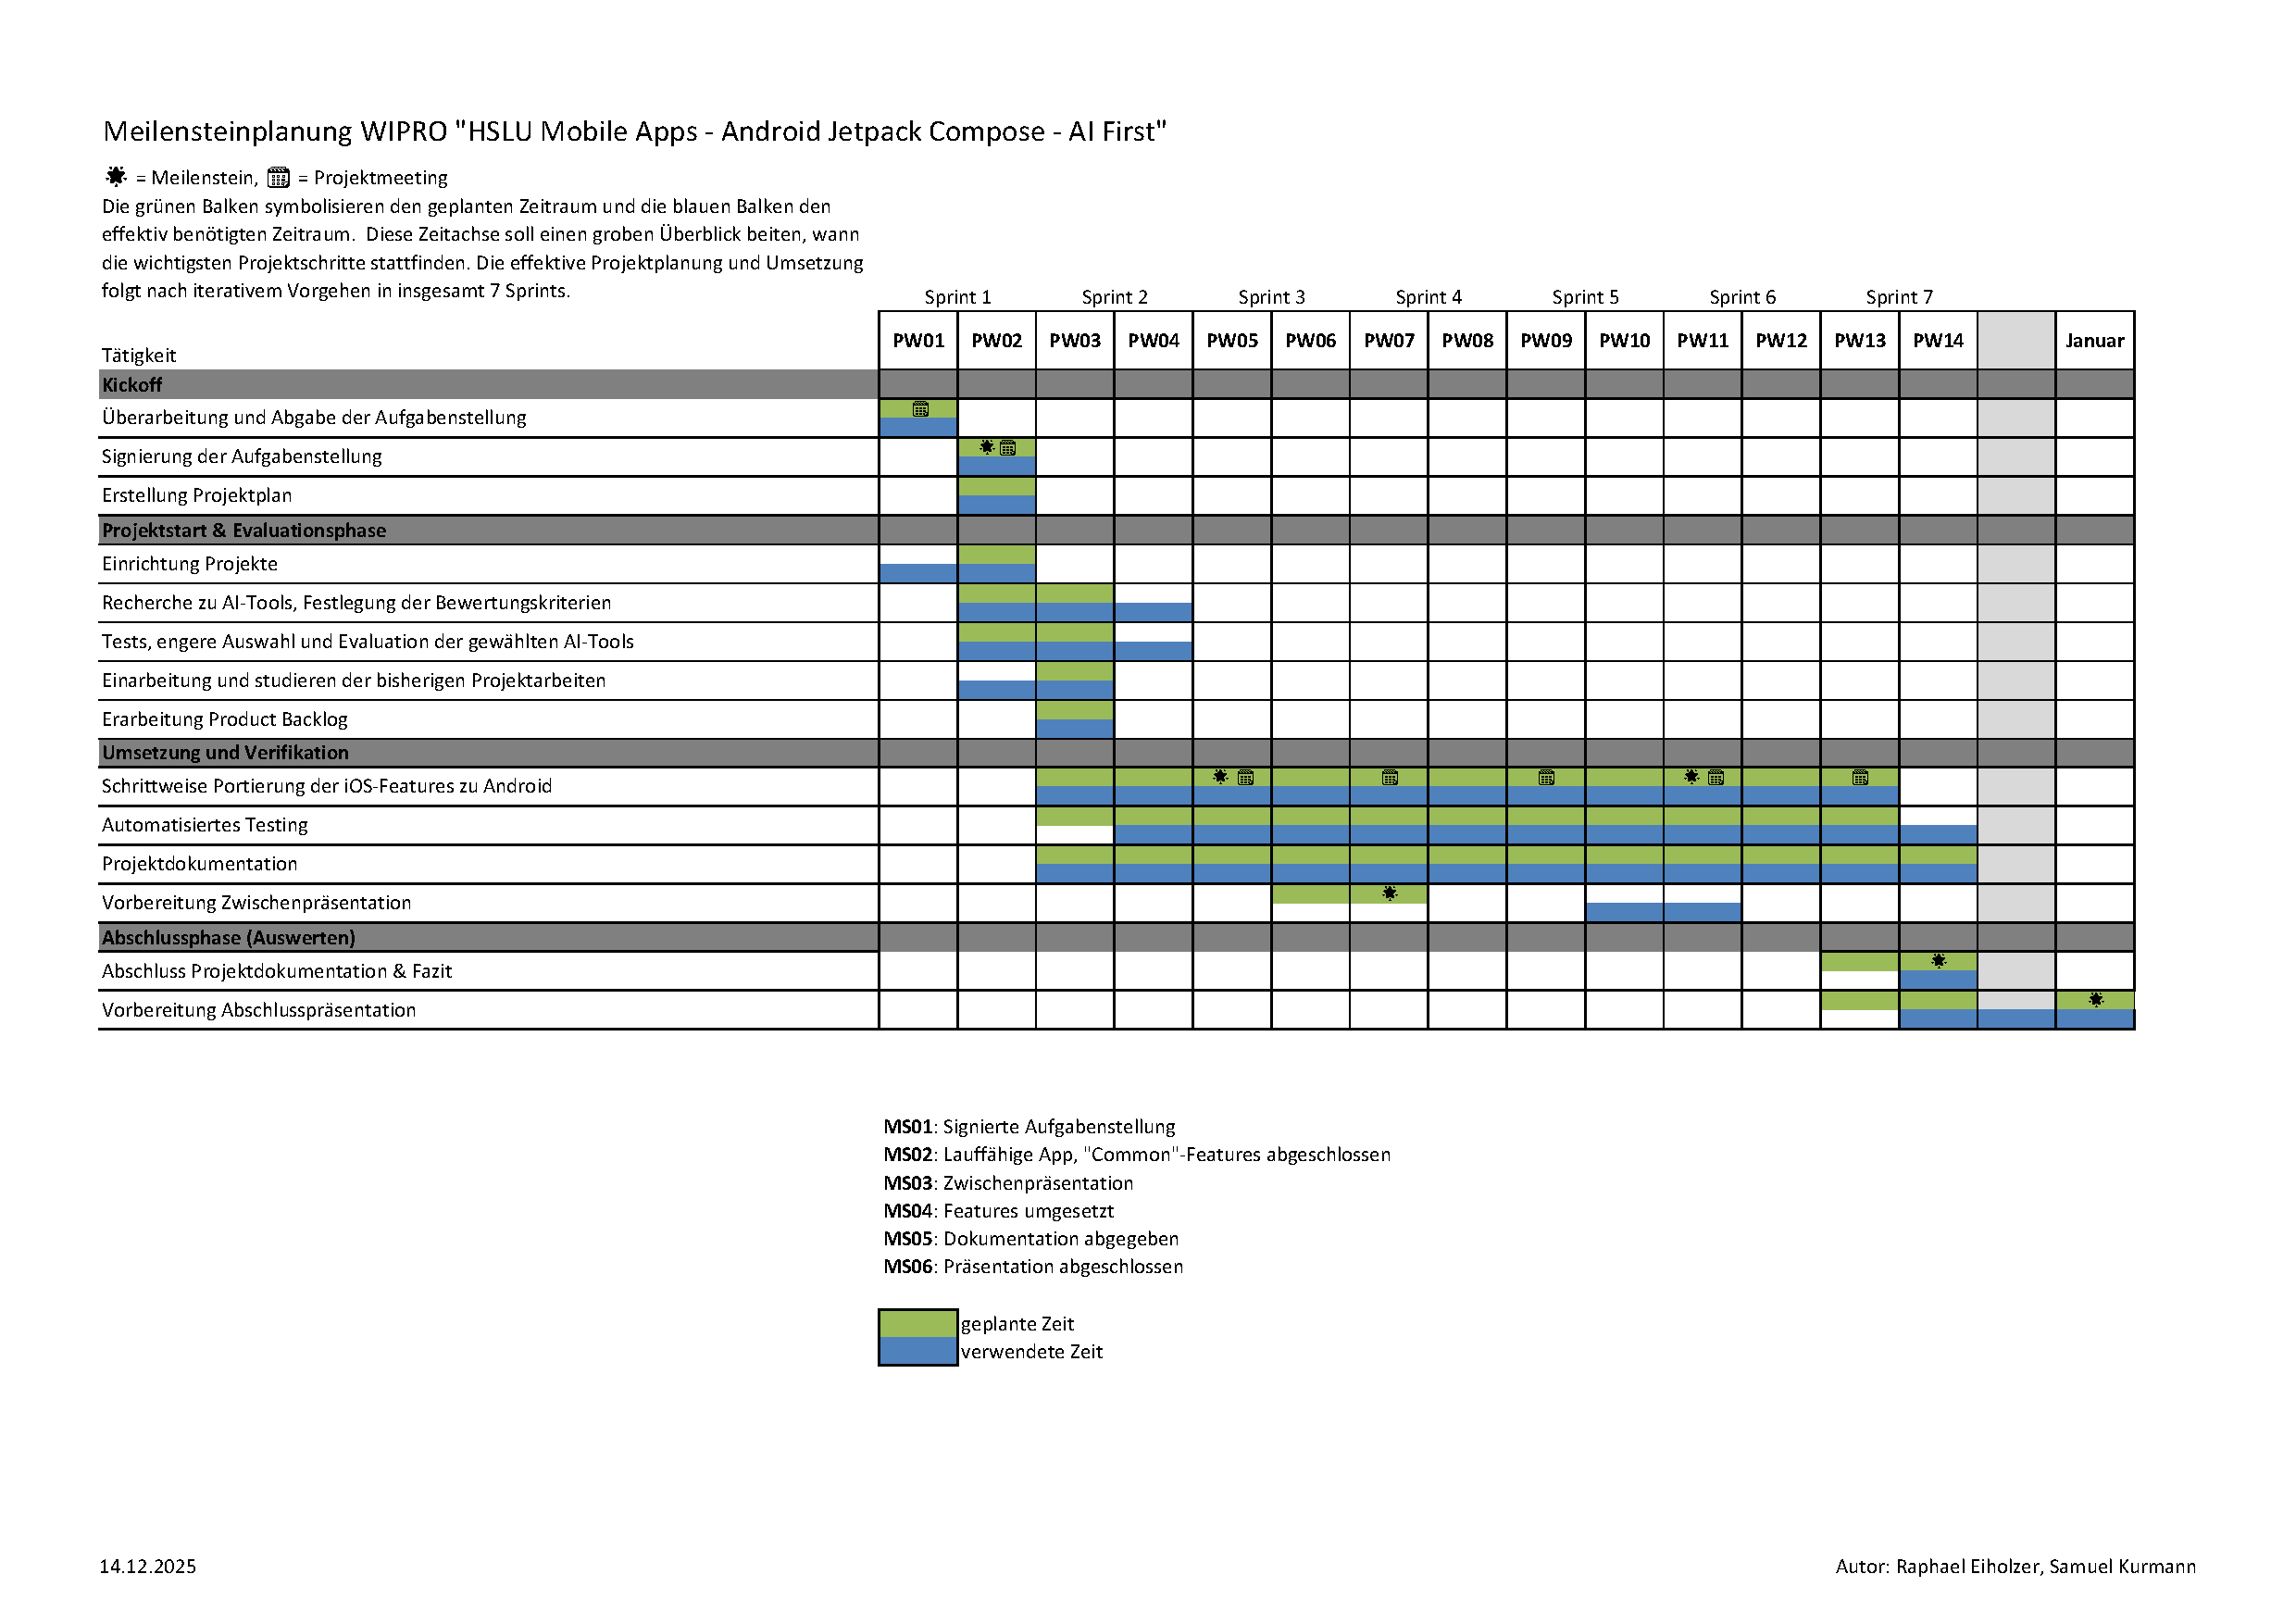
\includegraphics[width=0.85\textwidth]{Fotos/zeitplan.png}
    \caption{Meilensteinplan des Projekts}
    \label{fig:meilensteinplan}
\end{figure}\newpage

\subsection{Agiles Vorgehen}
Die Umsetzung des Projekts erfolgte nach einem agilen Vorgehen, angelehnt an
Scrum. Die Arbeit wurde in zweiwöchige Sprints unterteilt, woraus sich insgesamt
sieben Sprints ergaben. Vor jedem Sprint wurde im Team gemeinsam besprochen,
welche Aufgaben im kommenden Zeitraum umgesetzt werden sollen und wer welche
Arbeiten übernimmt.

\begin{figure}[H]
    \centering
    \includegraphics[width=0.35\textwidth]{Fotos/sprint_cycle.png}
    \caption{Darstellung des Scrum-Prozesses im Projekt} \parencite{atlassian_atlassian_nodate}
    \label{fig:scrum}
\end{figure}

Dieses Vorgehen ermöglichte ein effizientes Arbeiten, da Aufgaben flexibel
verteilt und bei freier Kapazität jederzeit neue Issues übernommen werden
konnten. Da alle Aufgaben und der aktuelle Projektstand in GitLab erfasst
waren, hatte auch der Auftraggeber jederzeit Einblick in den Fortschritt des
Projekts.

Zur Nachvollziehbarkeit des Projektverlaufs sind die Sprint-Backlogs als
grafische Übersicht im Anhang dokumentiert und zeigen den Fortschritt über die
gesamte Projektdauer hinweg (siehe ~\ref{anhang:sprintboard-1}).

\vspace{1.0em}
\begin{figure}[H]
    \centering
    \includegraphics[width=0.99\textwidth]{Fotos/sprintplanung-1.png}
    \caption{Backlogs in GitLab zu Projektbeginn}
    \label{fig:backlog}

\end{figure}\newpage

\subsubsection{Issues}
Alle Aufgaben im Projekt wurden als Issues in GitLab erfasst. Diese wurden
meist als einfache User Stories formuliert und mit einer kurzen
\textit{Definition of Done} (DoD) ergänzt. Dadurch war von Beginn an klar,
was zu einer Aufgabe gehört und wann sie als abgeschlossen gilt. Dies half, 
die Anforderungen besser zu verstehen und Missverständnisse zu
vermeiden.

Für jede Aufgabe wurde die aufgewendete Zeit direkt im jeweiligen Issue
dokumentiert. So konnte der Arbeitsaufwand über die gesamte Projektlaufzeit
hinweg nachvollzogen werden und es war jederzeit ersichtlich, wie viel Zeit
in welche Themen investiert wurde (siehe Anhang~\ref{anhang:zeit}).

\begin{figure}[H]
    \centering
    \includegraphics[width=0.7\textwidth]{Fotos/issue-userstory-dod.png}
    \caption{Beispiel einer User Story mit Definition of Done (DoD)}
    \label{fig:userstory}
\end{figure}

\subsection{Eingesetzte Programme/Tools}
Während der Projektdauer wurden diese Programme und Tools genutzt, um die Entwicklung, 
Dokumentation und die Organisation des Projekts zu unterstützen.

\vspace{0.6em}
\begin{table}[H]
\centering
\begin{tabular}{|l|p{12cm}|}
\hline
\textbf{Werkzeug} & \textbf{Einsatz im Projekt} \\
\hline
Git & Versionsverwaltung des Quellcodes \\
\hline
GitLab & Issue-Tracking, Sprint-Planung und Projektübersicht \\
\hline
OneNote & Persönliche Notizen, Skizzen und Screenshots während der Entwicklung \\
\hline
OneDrive & Zentrale Ablage für Projektdokumente und organisatorische Dateien \\
\hline
Latex & Erstellung und Formatierung der Projektdokumentation \\
\hline
VS Code & Editor zur Erstellung der Dokumentation \\
\hline
GitHub & Hosting des Dokumentations-Quellcodes \\
\hline
Android Studio & Endwicklungsumgebung für die Android-Applikation \\
\hline
Cursor & Endwicklungsumgebung mit AI-Features \\
\hline
Microsoft Teams & Kommunikation im Team und Meetings mit dem Auftraggeber \\
\hline
\end{tabular}
\caption{Eingesetzte Werkzeuge im Projekt}
\label{tab:werkzeuge}
\end{table}\clearpage


\subsection{Risikomanagement}
Zu Beginn des Projekts wurde eine Risikoanalyse erstellt, um die grössten Risiken frühzeitig zu identifizieren und entsprechende Gegenmassnahmen zu planen.  
Die Risiken wurden jeweils hinsichtlich Eintrittswahrscheinlichkeit und Auswirkung bewertet.  
Das Produkt dieser beiden Faktoren bestimmte den Gesamtrisiko-Wert und erlaubte es, die kritischsten Risiken zu priorisieren.  

Für jedes Risiko wurden präventive Massnahmen festgelegt, um die Eintrittswahrscheinlichkeit oder die Auswirkungen zu minimieren.  
Nach Umsetzung dieser Massnahmen wurde die Bewertung erneut vorgenommen, um verbleibende Risiken zu identifizieren und ihre Entwicklung über die Projektlaufzeit zu beobachten.  

\begin{figure}[H]
    \centering
    \includegraphics[width=0.4\textwidth]{Fotos/risikomatrix.png}
    \caption{Risikoanalyse und Risikomatrix des Projekts}
    \label{fig:risikomatrix}
\end{figure}

Die Risikoanalyse wurde während der gesamten Projektdauer regelmässig überprüft und aktualisiert.  
Am Ende jedes Sprints wurde die aktuelle Risikosituation besprochen und mögliche Massnahmen eingeleitet.  
Die drei grössten Risiken wurden zusätzlich an den Auftraggeber übermittelt, um Transparenz über den Projektfortschritt und potenzielle Herausforderungen sicherzustellen.
Die gesamte Risikoanalyse ist im Anhang zu finden (siehe Anhang~\ref{anhang:risk}).
\newpage

\chapter{Realisierung}
% Erläutere die Umsetzung, Architektur, Implementierungsdetails usw.

% Grundeinstellung App

\section*{Einleitung}

Das Ziel der Entwicklung war es, eine modulare und erweiterbare Applikation zu schaffen. 
Dazu wurde auf die bestehende iOS-Projektstruktur aufgebaut und das Android-Projekt analog dazu umgesetzt. 

Im Wesentlichen wurde die Anwendung in die beiden Hauptmodule \texttt{common} und \texttt{features} gegliedert:
\begin{itemize}
    \item \textbf{common}: Enthält alle allgemeinen und wiederverwendbaren Komponenten, wie z.\,B. UI-Elemente, Utility-Klassen und grundlegende Architekturbausteine.
    \item \textbf{features}: Beinhaltet die einzelnen Funktionsmodule der App, die jeweils auf spezifische Anwendungsbereiche oder Features ausgerichtet sind.
\end{itemize}

Dabei gilt die Abhängigkeitsregel, dass \texttt{features}-Module auf Inhalte aus \texttt{common} zugreifen dürfen, 
nicht jedoch umgekehrt – um zirkuläre Abhängigkeiten und eine enge Kopplung zu vermeiden.

\vspace{1em}

\begin{figure}[H]
    \centering
    \includegraphics[width=0.375\textwidth]{Fotos/projektexplorer_androidstudio.png}
    \caption{Projektstruktur im Android Studio}
    \label{fig:projektstruktur_androidstudio}
\end{figure}
\subsection{Lokalisierung}

Die App ist so konzipiert, dass sie in mehreren Sprachen verfügbar ist
(aktuell Deutsch und Englisch). Eine grundlegende Lokalisierungslogik war
bereits im ursprünglichen Android-Projekt vorhanden und wurde im Rahmen
dieses Projekts weiterentwickelt.

Die Lokalisierung basiert weiterhin auf dem standardmässigen
Android-Resource-System. (Android wählt automatisch die passende strings.xml 
basierend auf dem System-Locale) 
Dieses System wurde zusätzlich so ergänzt, dass auch
dynamisch geladene Inhalte (beispielsweise Menüpunkte aus dem
Bootstrapping-Prozess) zur Laufzeit korrekt lokalisiert dargestellt
werden können.

\subsubsection*{Konzept}
\begin{itemize}
    \item Die Sprachauswahl erfolgt automatisch über die Systemeinstellung
    des Geräts; eine separate Auswahl der App-Sprache ist nicht vorgesehen.
    \item Es wird ein ressourcenbasiertes Lokalisierungskonzept verwendet:
    Deutsch ist als Standardsprache im Ordner \texttt{values/} hinterlegt,
    Englisch im Ordner \texttt{values-en/}. Diese Ordner existieren jeweils
    pro Feature-Modul.
    \item Die Verwendung von UI-Strings erfolgt Android-typisch über
    \texttt{stringResource(R.string.\dots)} in Compose beziehungsweise über
    \texttt{context.getString(\dots)}.
\end{itemize}

\hspace{0.3cm}

\begin{lstlisting}[language=XML, caption={Default (Deutsch) und Englisch in \texttt{strings.xml}}]
<!-- values/strings.xml -->
<string name="Roomsearch_NavItem">Raumsuche</string>
<string name="Settings_NavItem">Einstellungen</string>

<!-- values-en/strings.xml -->
<string name="Roomsearch_NavItem">Roomsearch</string>
<string name="Settings_NavItem">Settings</string>
\end{lstlisting}

\subsubsection*{Übersetzung dynamischer Inhalte}
Für dynamisch geladene Inhalte, wie beispielsweise Menüpunkte aus
Remote-DTOs (siehe Abschnitt~\ref{sec:featureappinit}), wird die Sprache zur Laufzeit 
anhand der aktuellen Systemsprache bestimmt. Die Auswahl erfolgt über \newline
\texttt{Locale.getDefault()} und ordnet die passenden Sprachfelder zu:

\hspace{0.3cm}

\begin{lstlisting}[language=Java, caption={Auswahl der passenden Sprachvariante}]
val label: String
    get() = when (Locale.getDefault().language.lowercase(Locale.getDefault())) {
        "de" -> LabelDE ?: LabelEN ?: "Unbenannt"
        else -> LabelEN ?: LabelDE ?: "Unnamed"
    }
\end{lstlisting}

(Es wird zuerst versucht, die aktuell gesetzte Systemsprache zu
verwenden. Ist für diese keine Übersetzung verfügbar, wird automatisch
auf die jeweils andere unterstützte Sprache zurückgegriffen. Sollte
auch diese nicht vorhanden sein, wird ein Fallback-Wert
(\textit{z.\,B.} \texttt{'Unnamed'}) verwendet.)

Damit sind alle Inhalte der App
vollständig auf Deutsch und Englisch verfügbar. Weitere Sprachen könnten
bei Bedarf einfach ergänzt werden, indem zusätzliche
\texttt{strings.xml}-Dateien angelegt werden. \newpage
\subsection{Fastlane}

Das Fastlane-Setup für die Android-App automatisiert den Build- und Deployment-Prozess für beide Tenants (HSLU I und HSLU TA). 
Anstatt separate Fastfiles pro Tenant zu verwenden wie das im Android-XML Projekt der Fall ist, wurde ein einheitliches, parametrisiertes Fastfile implementiert, 
das Redundanzen eliminiert und die Wartbarkeit verbessert. Das Fastfile unterstützt Debug- und Release-Builds sowie automatische Uploads zu Google Play Store in verschiedenen Tracks (Beta, Internal, Production).

\subsubsection*{Ziel und Motivation}

Das Hauptziel besteht darin, die CI/CD-Pipeline zu vereinfachen und Redundanzen zu eliminieren. 
Durch die Parametrisierung mit dem \texttt{tenant}-Parameter kann ein einziges Fastfile für beide Tenants verwendet werden, 
was die Wartbarkeit erheblich verbessert. Zusätzlich werden alle sensiblen Daten (Keystores, API-Keys) sicher in einem separaten Git-Repository gespeichert und verschlüsselt, 
sodass sie nicht im Haupt-Repository liegen.

Ein weiteres wichtiges Ziel ist die Automatisierung des gesamten Build- und Deployment-Prozesses, 
von der Kompilierung über die Signierung bis hin zum Upload in den Google Play Store. 
Dies reduziert manuelle Fehler und beschleunigt den Release-Prozess erheblich.

\subsubsection*{Umsetzung / Funktionsweise}

Die Implementierung basiert auf einem zentralen \texttt{before\_all}-Block, der die Initialisierung und Konfiguration für alle Lanes übernimmt. 
Das Fastfile verwendet Dotenv für die Verwaltung von Secrets und parametrisiert alle tenant-spezifischen Werte. 
Der \texttt{before\_all}-Block wird vor jeder Lane ausgeführt und übernimmt die Validierung des \texttt{tenant}-Parameters, 
die Definition von Pfaden sowie das Mapping von Tenant-Namen zu Android-Modulen und Package-IDs.

Die tenant-spezifischen Umgebungsvariablen (Keystore-Passwörter, API-Keys, etc.) werden aus \texttt{.env.secret} geladen 
und in generische Variablen gemappt, sodass alle Lanes die gleichen Variablennamen verwenden können.

\paragraph*{Lanes}

Das Fastfile definiert vier Haupt-Lanes, die in der folgenden Tabelle beschrieben sind:

\begin{table}[h]
\centering
\begin{tabularx}{\textwidth}{|l|X|}
\hline
\textbf{Lane} & \textbf{Beschreibung} \\
\hline
\texttt{build\_debug} & Erstellt einen Debug-Build ohne Signierung. Führt \texttt{gradle clean assemble} für das entsprechende Tenant-Modul aus und kopiert die Artefakte in den Output-Ordner. Wird hauptsächlich für lokale Tests verwendet. \\
\hline
\texttt{build\_release} & Erstellt einen signierten Release-Build. Lädt den verschlüsselten Keystore aus dem Zertifikats-Repository, entschlüsselt ihn, erstellt die \texttt{keystore.properties}-Datei für Gradle und führt \texttt{gradle clean bundle} aus. Das signierte AAB wird in den Output-Ordner kopiert. \\
\hline
\texttt{beta} & Baut ein signiertes Release-Bundle und lädt es in den Google Play Store hoch. Standardmässig wird der Beta-Track verwendet, kann aber über den \texttt{track:}-Parameter überschrieben werden (z.\,B. \texttt{track:internal}). Lädt sowohl Keystore als auch Google Play API-Key aus dem Zertifikats-Repository. Ruft intern \texttt{build\_release} auf und lädt anschliessend das AAB hoch. \\
\hline
\texttt{release} & Analog zu \texttt{beta}, lädt jedoch explizit in den Production-Track des Google Play Stores. Wird für finale Releases verwendet. \\
\hline
\end{tabularx}
\caption{Übersicht der Fastlane-Lanes}
\label{tab:fastlane-lanes}
\end{table}

\paragraph*{Hilfsfunktionen}

Das Fastfile verwendet mehrere Hilfsfunktionen zur Verwaltung von Zertifikaten und Konfiguration:

\begin{itemize}
    \item \texttt{download\_from\_certs\_repo}: Klont das Zertifikats-Repository und entschlüsselt eine Datei (typischerweise den Keystore) mit OpenSSL (AES-256-CBC).
    \item \texttt{download\_from\_certs\_repo\_full}: Erweiterte Variante, die sowohl Keystore als auch Google Play API-Key entschlüsselt.
    \item \texttt{create\_keystore\_properties}: Erstellt die \texttt{keystore.properties}-Datei dynamisch, die von Gradle für die Signierung verwendet wird.
    \item \texttt{clean\_directory}: Entfernt temporäre Zertifikatsdateien nach dem Build, um Sicherheitsrisiken zu minimieren.
\end{itemize}

\subsubsection*{Verwendung und Sicherheit}

Die Verwendung erfolgt durch Aufruf von Fastlane mit dem \texttt{tenant}-Parameter: 
\texttt{fastlane <lane> tenant:hslui} oder \texttt{fastlane <lane> tenant:hsluta}. 
Ohne diesen Parameter bricht Fastlane mit einer Fehlermeldung ab.

Alle sensiblen Daten (Keystores, API-Keys) werden in einem separaten Git-Repository gespeichert und mit OpenSSL verschlüsselt (AES-256-CBC). 
Die Passwörter für die Entschlüsselung werden aus \texttt{.env.secret} geladen, das nicht im Repository gespeichert wird, 
sondern von der CI/CD-Pipeline zur Laufzeit erstellt wird. Die Keystore-Properties-Datei wird dynamisch erstellt 
und nach dem Build gelöscht, um Sicherheitsrisiken zu minimieren.

Die Upload-Funktionalität unterstützt verschiedene Tracks im Google Play Store. 
Der Standard-Track für \texttt{beta} ist "beta", kann aber über den \texttt{track:}-Parameter überschrieben werden (z.\,B. \texttt{track:internal}). 
Changelogs werden bewusst übersprungen, da diese manuell im Google Play Console verwaltet werden.

Das Fastfile ist erweiterbar für weitere Tenants, indem einfach ein neuer \texttt{when}-Fall im 
\texttt{before\_all}-Block hinzugefügt wird und die entsprechenden Umgebungsvariablen in \texttt{.env.secret} definiert werden.
 \newpage

% Common
\section{Common-Komponenten} \label{sec:common}
\subsection{CommonApplication}

Das Common Application Modul stellt die zentrale Anwendungsschicht für die modulare Multi-Tenant Android-Anwendung dar. 
Es implementiert eine generische, wiederverwendbare Architektur für das Laden, Synchronisieren und Verwalten von Feature-Modulen über verschiedene Datenquellen hinweg. 
Die Kernkomponente ist die abstrakte Basisklasse \texttt{CommonApplicationBaseModuleLoader}, die von allen Feature-Modulen erweitert wird.

\subsubsection*{Ziel und Motivation}

Das Hauptziel besteht darin, Code-Duplikation zu vermeiden und eine konsistente Datenlade- und Synchronisationslogik über alle Feature-Module hinweg zu gewährleisten. 
Durch eine abstrakte Basisklasse, die den gesamten Datenlade- und Synchronisationsprozess kapselt, 
müssen konkrete Feature-Module nur noch ihre spezifischen Typparameter und Konfigurationen bereitstellen. 
Dies reduziert den Implementierungsaufwand erheblich und stellt sicher, dass alle Module die gleichen Qualitätsstandards in Bezug auf Fehlerbehandlung, 
Offline-Funktionalität und Performance-Optimierungen einhalten.

Ein weiteres wichtiges Ziel ist die Implementierung einer intelligenten Synchronisationsstrategie,
 die sowohl Bandbreite als auch Batterie schont. Durch den Vergleich von lokalen und remote Timestamps wird nur dann eine Aktualisierung durchgeführt, 
 wenn tatsächlich neue Daten verfügbar sind, was eine Offline-First-Architektur ermöglicht.

\subsubsection*{Umsetzung / Funktionsweise}

Die Umsetzung basiert auf dem Template-Method-Pattern mit generischen Typparametern. 
Die Basisklasse verwendet drei Typparameter: \texttt{I} für den Item-Typ, \texttt{T} für den Container-Typ und 
\texttt{C} für den Konfigurationstyp.
Die vollständige Klassendefinition findet sich in \texttt{CommonApplicationBaseModuleLoader.kt}, Zeilen 26-28.

Der Loader verwaltet seinen Zustand über einen \texttt{StateFlow<CommonModuleLoaderStatus<I>>}, der verschiedene Zustände unterstützt: 
\texttt{Not\_Initialized}, \texttt{Initialized}, \texttt{Processing}, \texttt{Success}, \texttt{Success\_Cached} und \texttt{ErrorOn}. 
Die \texttt{process()}-Methode orchestriert den gesamten Datenladevorgang und wählt basierend auf dem \texttt{moduleLoaderType} die entsprechende Strategie.
Die vollständige Implementierung der \texttt{process()}-Methode findet sich in \texttt{CommonApplicationBaseModuleLoader.kt}, Zeilen 52-77.

Der Hybrid-Modus implementiert eine intelligente Synchronisationslogik, die auf Timestamp-Vergleichen basiert. 
Zuerst wird über die Sync-URL ein JSON-Objekt abgerufen, das das Feld \texttt{ModuleLastUpdated} enthält. 
Gleichzeitig wird versucht, den lokalen Timestamp aus der Room-Datenbank zu laden. 
Die Entscheidungslogik vergleicht diese beiden Timestamps.
Die vollständige Timestamp-Vergleichslogik findet sich in \texttt{CommonApplicationBaseModuleLoader.kt}, Zeilen 151-157.

Wenn eine Aktualisierung notwendig ist, werden die Daten heruntergeladen und mit Gson deserialisiert. 
Dabei wird ein \texttt{TypeToken} verwendet, um die korrekte Generik-Auflösung zur Laufzeit zu gewährleisten.
Die Gson-Deserialisierung findet sich in \\ \texttt{CommonApplicationBaseModuleLoader.kt}, Zeilen 169-172.

Nach erfolgreichem Parsing wird überprüft, ob die Daten gespeichert werden sollen. 
Die \texttt{shouldStoreData()}-Methode kann von Subklassen überschrieben werden, um bestimmte Datentypen nicht zu speichern. 
Wenn die Daten gespeichert werden sollen, werden sie zusammen mit dem \texttt{lastUpdated}-Timestamp als \texttt{ModuleDataEntity} in der Room-Datenbank gespeichert.

\subsubsection*{Spezifische Infos}

Die folgende Tabelle gibt einen Überblick über die wichtigsten technischen Aspekte \\ des \texttt{CommonApplicationBaseModuleLoader}:

\begin{table}[h]
\centering
\begin{tabularx}{\textwidth}{|l|X|}
\hline
\textbf{Aspekt} & \textbf{Beschreibung} \\
\hline
\textbf{Dependency Injection} & 
Die Integration mit Feature-Modulen erfolgt über Dependency Injection mit Dagger Hilt. 
Ein konkretes Feature-Modul wie \texttt{MensaModuleLoader} erbt von \texttt{CommonApplicationBaseModuleLoader} und spezifiziert die Typparameter \texttt{I}, \texttt{T} und \texttt{C}. 
Die vollständige Implementierung des \texttt{MensaModuleLoader} findet sich in \texttt{MensaModuleLoader.kt}, Zeilen 16-31. \\
\hline
\textbf{UI-Integration} & 
In ViewModels oder Composables kann der Loader direkt verwendet werden. Der \texttt{loadingStatus} wird als \texttt{StateFlow} bereitgestellt und kann mit \texttt{collectAsState()} beobachtet werden, um reaktive UI-Updates zu ermöglichen. 
Die \texttt{process()}-Methode wird typischerweise in einem \texttt{LaunchedEffect} aufgerufen. \\
\hline
\textbf{Asynchrone Operationen} & 
Alle asynchronen Operationen werden über Kotlin Coroutines abgewickelt. Der Loader erbt von \texttt{ViewModel}, was automatisch einen \texttt{viewModelScope} bereitstellt, der alle Coroutines automatisch abbricht, wenn das ViewModel zerstört wird. 
Netzwerk- und Speicheroperationen werden explizit auf \texttt{Dispatchers.IO} ausgeführt, um den Main-Thread nicht zu blockieren. \\
\hline
\textbf{Fehlerbehandlung} & 
Die Fehlerbehandlung ist mehrschichtig implementiert: 
\begin{itemize}[leftmargin=*,nosep]
    \item Netzwerk-Fehler werden durch \texttt{networkService.hasConnection()} und \texttt{isRemoteReachable()} erkannt
    \item Parse-Fehler werden durch try-catch-Blöcke bei der Gson-Deserialisierung abgefangen
    \item Speicher-Fehler werden bei Room-Datenbankoperationen abgefangen und geloggt
\end{itemize} \\
\hline
\textbf{Performance-Optimierungen} & 
Performance-Optimierungen umfassen Lazy Loading, Caching in der Room-Datenbank und inkrementelle Updates, wobei nur bei geänderten Timestamps Daten neu geladen werden. 
Die Offline-First-Strategie stellt sicher, dass lokale Daten Priorität haben, wenn keine Netzwerkverbindung verfügbar ist. \\
\hline
\end{tabularx}
\caption{Technische Aspekte des \texttt{CommonApplicationBaseModuleLoader}}
\label{tab:commonapplication-specs}
\end{table} \newpage
\subsection{CommonDomain}

Das Common Domain Module stellt die Domänenschicht der Anwendung dar und enthält alle zentralen Geschäftsobjekte, 
Data Transfer Objects (DTOs), Enums und Konfigurationsklassen, die die Kernentitäten der Anwendung repräsentieren. 
Es handelt sich um ein reines Domänenmodul ohne Abhängigkeiten zu Android-Frameworks, 
das den Prinzipien der Clean Architecture folgt und eine klare Trennung zwischen Domänenlogik und Infrastruktur ermöglicht.

\subsubsection*{Ziel und Motivation}

Das Hauptziel des Common Domain Modules besteht darin, eine zentrale Domänenschicht zu schaffen, 
die von allen anderen Modulen verwendet werden kann, ohne direkte Abhängigkeiten zu Infrastruktur- oder Anwendungsschichten zu haben. 
Dies ermöglicht eine saubere Architektur, bei der Geschäftsobjekte unabhängig von ihrer konkreten Implementierung definiert werden können. 
Durch die Verwendung von DTOs für die API-Kommunikation wird eine klare Schnittstelle zwischen der Anwendung und externen Datenquellen geschaffen.

Ein weiteres wichtiges Ziel ist die Vermeidung von Code-Duplikation durch die Bereitstellung von Basisklassen wie 
\texttt{CommonAppBaseModuleItemAPIDTO} und \texttt{CommonAppBaseModuleAPIDTO}, die von allen Feature-spezifischen DTOs erweitert werden können. 
Dies stellt sicher, dass alle Module eine konsistente Datenstruktur verwenden und gemeinsame Funktionalität zentralisiert wird.

\subsubsection*{Umsetzung / Funktionsweise}

Die Struktur des Moduls basiert auf einer klaren Trennung in verschiedene Pakete: \texttt{dto} für Data Transfer Objects, 
\texttt{enums} für Aufzählungstypen, \texttt{config} für Konfigurationsklassen, \texttt{loader} für Loader-Interfaces und 
\texttt{protocols} für Protokoll-Definitionen.

Die Basis-DTOs definieren die gemeinsame Struktur für alle Modul-DTOs. \texttt{CommonAppBaseModuleItemAPIDTO} stellt die Basis für einzelne Modul-Items dar.
Die vollständige Definition findet sich in \texttt{CommonAppBaseModuleDTOs.kt}, Zeilen 5-8.

\texttt{CommonAppBaseModuleAPIDTO} ist ein generischer Container für Modul-Daten, der sowohl einzelne Items als auch Listen unterstützt.
Die vollständige Definition findet sich in \texttt{CommonAppBaseModuleDTOs.kt}, Zeilen 10-21.

Feature-spezifische DTOs erben von diesen Basisklassen. Beispielsweise erbt \texttt{AppMensaModuleItemAPIDTO} von 
\texttt{CommonAppBaseModuleItemAPIDTO} und fügt mensa-spezifische Felder hinzu. 
Die Verwendung von Gson-Annotationen wie \texttt{@SerializedName} ermöglicht die korrekte Deserialisierung von JSON-Daten aus der API.

Die Enum-Klassen definieren verschiedene Zustände und Typen der Anwendung. \texttt{CommonModuleLoaderStatus} ist eine sealed class, 
die alle möglichen Zustände eines Modul-Loaders repräsentiert.
Die vollständige Definition der sealed class findet sich in \texttt{CommonModuleLoaderStatus.kt}, Zeilen 5-12.

\texttt{CommonAppModuleType} definiert alle verfügbaren Modultypen der Anwendung.
Die vollständige Enum-Definition mit der \texttt{parse()}-Methode findet sich in \texttt{CommonAppModuleType.kt}, Zeilen 7-35.

Die Konfigurationsklassen definieren die Einstellungen für verschiedene Module. 
\texttt{CommonModuleBaseLoaderConfig} stellt die Basis-Konfiguration für Modul-Loader bereit.
Die vollständige Konfigurationsklasse findet sich in \\ \texttt{CommonModuleBaseLoaderConfig.kt}, Zeilen 6-13.

Das \texttt{ModuleLoaderContract} Interface definiert den Vertrag für alle Modul-Loader.
Die vollständige Interface-Definition findet sich in \texttt{CommonModuleLoaderTypes.kt}, Zeilen 7-10.

\subsubsection*{Spezifische Infos}

Die folgende Tabelle gibt einen Überblick über die wichtigsten technischen Aspekte des \texttt{CommonDomain} Moduls:

\begin{table}[h]
\centering
\begin{tabularx}{\textwidth}{|l|X|}
\hline
\textbf{Aspekt} & \textbf{Beschreibung} \\
\hline
\textbf{Abhängigkeiten} & 
Das Modul hat minimale Abhängigkeiten: \texttt{androidx.core:core-ktx} für Android Core Utilities, \texttt{com.google.code.gson:gson} für JSON-Serialisierung und \texttt{kotlinx-coroutines-core} für Coroutines-Unterstützung. 
Dies stellt sicher, dass das Modul keine Android-spezifischen Abhängigkeiten hat und theoretisch auch in anderen Kontexten verwendet werden könnte. \\
\hline
\textbf{Gson-Annotationen} & 
Die DTOs verwenden Gson-Annotationen für die Serialisierung und Deserialisierung. Die \texttt{@SerializedName}-Annotation ermöglicht es, JSON-Feldnamen zu mappen, die nicht den Kotlin-Namenskonventionen entsprechen. 
Dies ist besonders wichtig bei der Integration mit externen APIs, die möglicherweise andere Namenskonventionen verwenden. \\
\hline
\textbf{Computed Properties} & 
Einige DTOs wie \texttt{AppInitModuleItemAPIDTO} enthalten computed properties, die basierend auf der aktuellen Locale die richtige Sprache auswählen. 
Die vollständige Implementierung der computed property findet sich in \texttt{AppInitModuleItemDTO.kt}, Zeilen 62-66. \\
\hline
\textbf{Sealed Classes} & 
Die Verwendung von sealed classes für Status-Enums ermöglicht exhaustive when-Ausdrücke in Kotlin, was die Typsicherheit erhöht und Compiler-Warnungen bei fehlenden Fällen auslöst. 
Dies verbessert die Code-Qualität und reduziert potenzielle Laufzeitfehler. \\
\hline
\textbf{Clean Architecture} & 
Das Modul folgt den Prinzipien der Clean Architecture, indem es keine Abhängigkeiten zu anderen Schichten hat. 
Alle anderen Module können das Domain-Modul verwenden, aber das Domain-Modul selbst hängt nur von Standard-Kotlin- und minimalen Android-Bibliotheken ab. 
Dies ermöglicht eine einfache Testbarkeit und Wartbarkeit des Codes. \\
\hline
\end{tabularx}
\caption{Technische Aspekte des \texttt{CommonDomain} Moduls}
\label{tab:commondomain-specs}
\end{table} \newpage

\subsection{CommonInfrastructure}
\subsubsection{Network}  \label{sec:commonnetwork}

Die Klasse CommonNetworkService stellt die zentrale Netzwerkschicht der Anwendung dar und bietet eine einheitliche Schnittstelle für alle Netzwerkoperationen. 
Es abstrahiert die Komplexität der Netzwerkkommunikation und bietet typsichere Methoden für HTTP-Requests, JSON-Parsing und Datei-Downloads. 
Die gesamte iOS Netzwerkarchitektur wurde auf Android migriert, wobei eine identische Architektur beibehalten wurde und gleiche Methodennamen sowie API-Struktur verwendet werden.
Es wurden moderne Android Best Practices verwendet wie Kotlin Coroutines, StateFlow für reaktives UI, Hilt Dependency Injection und eine Type-safe API mit Compile-Time-Checks.
Der Multitenant-Ansatz wurde berücksichtigt, sodass je nach Build-Varianten die korrekten URLs und Tokens verwendet werden, wodurch Redundanzen verhindert werden konnten.

\subsubsection*{Ziel und Motivation}

Das Hauptziel besteht darin, eine zentrale, wiederverwendbare Netzwerkschicht zu schaffen, die von allen Feature-Modulen verwendet werden kann, 
ohne dass jedes Modul seine eigene Netzwerk-Implementierung benötigt. Durch die Verwendung von Kotlin Coroutines und suspend-Funktionen wird eine moderne, 
asynchrone API bereitgestellt, die den Main-Thread nicht blockiert und eine reaktive Programmierung ermöglicht.

Die Verwendung von Hilt für Dependency Injection ermöglicht eine saubere Trennung von Konfiguration und Implementierung, 
während der Multitenant-Ansatz sicherstellt, dass verschiedene Build-Varianten (hslui, hsluta) automatisch die korrekten URLs und Tokens verwenden.

\subsubsection*{Umsetzung / Funktionsweise}

Die Implementierung basiert auf Android's HTTP-Client-Bibliotheken und Kotlin Coroutines. 
Der \newline \texttt{CommonNetworkService} ist die zentrale Service-Klasse, die alle Netzwerkoperationen kapselt:

\begin{lstlisting}[language=Kotlin, caption={Klasse CommonNetworkService}]
class CommonNetworkService(
    private val httpClient: OkHttpClient,
    private val tenantUrlProvider: TenantUrlProvider
) {
    suspend fun getAsJsonObject(url: String): JsonObject?
    // ...
}
\end{lstlisting}

Der \texttt{NetworkMonitor} überwacht die Netzwerkverbindung und stellt Informationen über die aktuelle Verbindungsqualität bereit. 
Die Implementierung verwendet Android's \texttt{ConnectivityManager} für die Erkennung von Netzwerkänderungen.

Die Tenant-Konfiguration ermöglicht es, verschiedene Build-Varianten mit unterschiedlichen URLs und Tokens zu verwenden:

\begin{table}[H]
\centering
\begin{tabular}{|c|c|c|c|}
\hline
\textbf{Tenant} & \textbf{Base URL} & \textbf{Client Token} & \textbf{Build Variant} \\
\hline
HSLU I & hslui.mobile-hslu.ch & xxxxxxxx-xxxx-xxxx-xxxx-xxxxxxxxxxxx & hslui \\
\hline
HSLU TA & hsluta.mobile-hslu.ch & yyyyyyy-yyyy-yyyy-yyyy-yyyyyyyyyyyy & hsluta \\
\hline
\end{tabular}
\caption{Tenant-Konfiguration für verschiedene Build-Varianten}
\label{tab:commonnetwork-tenants}
\end{table}

\subsubsection*{Weitere Informationen}

\begin{table}[h]
\centering
\begin{tabularx}{\textwidth}{|l|X|}
\hline
\textbf{Aspekt} & \textbf{Beschreibung} \\
\hline
\textbf{Asynchrone Operationen} & 
Alle Netzwerkoperationen werden asynchron über Kotlin Coroutines ausgeführt. Die Verwendung von suspend-Funktionen stellt sicher, dass alle Operationen nicht-blockierend sind und den Main-Thread nicht beeinträchtigen. 
Dies ermöglicht eine reaktive Programmierung und verbessert die Performance der Anwendung. \\
\hline
\textbf{Type-Safe API} & 
Die API ist type-safe mit Compile-Time-Checks. Methoden wie \texttt{getAsJsonObject()}, \texttt{getAsJsonString()} und \texttt{getAsDownload()} bieten typsichere Rückgabewerte und reduzieren Laufzeitfehler. \\
\hline
\textbf{Multitenant-Unterstützung} & 
Der Multitenant-Ansatz wird durch \texttt{TenantUrlProvider} und tenant-spezifische Implementierungen unterstützt. 
Je nach Build-Variant werden automatisch die korrekten URLs und Tokens verwendet, wodurch Redundanzen verhindert werden. \\
\hline
\textbf{StateFlow für reaktives UI} & 
StateFlow wird für reaktives State-Management verwendet, ähnlich wie \texttt{@Published} in SwiftUI. 
Dies ermöglicht es, UI-Komponenten reaktiv auf Netzwerkstatusänderungen zu reagieren. \\
\hline
\end{tabularx}
\caption{Technische Aspekte des \texttt{CommonNetwork} Moduls}
\label{tab:commonnetwork-specs}
\end{table}

\hspace{1.00cm} \newpage
\subsubsection{CommonStorage}  \label{sec:commonstorage}

Das Common Storage Modul stellt die zentrale Speicherschicht der Anwendung dar und bietet eine einheitliche Schnittstelle für persistente Datenspeicherung. 
Es verwendet Android's Room-Datenbank als Backend und abstrahiert alle Datenbankoperationen hinter einem einfachen Service-Interface. 
Der \texttt{CommonStorageService} ermöglicht es, verschiedene Arten von Daten zu speichern: AppInitModule-Konfigurationen, Modul-JSON-Daten,  
Synchronisations-Timestamps und Dateien.

\subsubsection*{Ziel und Motivation}

Das Hauptziel besteht darin, eine zentrale, wiederverwendbare Speicherlösung zu schaffen, die von allen Feature-Modulen verwendet werden kann, 
ohne dass jedes Modul seine eigene Datenbank-Implementierung benötigt. Durch die Verwendung von Room als Backend wird eine robuste, 
typsichere und performante Datenbankzugriffsschicht bereitgestellt, die automatisch SQL-Abfragen generiert und Compile-Zeit-Validierung bietet.

Ein weiteres wichtiges Ziel ist die Abstraktion der Datenbankkomplexität. Anstatt dass jedes Modul direkt mit Room-Entities und DAOs arbeitet, 
bietet der \texttt{CommonStorageService} eine einfache, suspend-Funktion-basierte API, die DTOs aus der Domänenschicht verwendet. 
Dies ermöglicht es, die Datenbank-Implementierung zu ändern, ohne dass die Anwendungsschicht betroffen ist.

Die Verwendung von Kotlin Coroutines für alle Datenbankoperationen stellt sicher, dass Blockierungen des Main-Threads vermieden werden und die Anwendung reaktionsfähig bleibt. 
Alle Operationen werden automatisch auf \texttt{Dispatchers.IO} ausgeführt, was eine optimale Performance gewährleistet.

\subsubsection*{Umsetzung / Funktionsweise}

Die Implementierung basiert auf Android's Room-Persistenzbibliothek. Die \texttt{AppDatabase} ist die zentrale Datenbankklasse, 
die alle Entities und DAOs verwaltet:

\begin{lstlisting}[language=Java]
@Database(
    entities = [ModuleDataEntity::class, FileEntity::class, ...],
    version = 1
)
abstract class AppDatabase : RoomDatabase() {
    abstract fun moduleDataDao(): ModuleDataDao
    // ...
}
\end{lstlisting}

Der \texttt{CommonStorageService} verwendet das Singleton-Pattern für die Datenbankinstanz und bietet eine Factory-Methode zur Erstellung.

Für die Speicherung von Modul-Daten wird die \texttt{ModuleDataEntity} verwendet, die JSON-Daten als String speichert:

\begin{lstlisting}[language=Java]
@Entity(tableName = "module_data")
data class ModuleDataEntity(
    @PrimaryKey val moduleId: String,
    val jsonData: String,
    val lastUpdated: String
)
\end{lstlisting}

Die \texttt{storeModuleData()}-Methode konvertiert DTOs in Entities und speichert sie in der Datenbank.

Die \texttt{getModuleData()}-Methode lädt Daten aus der Datenbank und gibt sie als JSON-String zurück.

Für AppInitModule-Daten werden DTOs in Entities konvertiert. Die \texttt{storeAppInitModules()}-Methode mappt eine Liste von DTOs zu Entities.

Die \texttt{getAppInitModuleOrder()}-Methode demonstriert eine komplexere Abfrage, 
die Daten aus mehreren Tabellen kombiniert.

Für Dateispeicherung wird die \texttt{FileEntity} verwendet, die Dateien als \texttt{ByteArray} speichert:

\begin{lstlisting}[language=Java]
@Entity(tableName = "files")
data class FileEntity(
    @PrimaryKey val fileId: String,
    val data: ByteArray,
    val mimeType: String
)
\end{lstlisting}

\subsubsection*{Weitere Informationen}

\begin{table}[h]
\centering
\begin{tabularx}{\textwidth}{|l|X|}
\hline
\textbf{Aspekt} & \textbf{Beschreibung} \\
\hline
\textbf{Asynchrone Operationen} & Alle Datenbankoperationen werden asynchron über Kotlin Coroutines ausgeführt. Die Verwendung von \texttt{withContext(Dispatchers.IO)} stellt sicher, dass alle Operationen auf dem IO-Dispatcher laufen und den Main-Thread nicht blockieren. Dies ist besonders wichtig für grössere Datenmengen oder komplexe Abfragen. \\
\hline
\textbf{Fehlerbehandlung} & 
Die Fehlerbehandlung erfolgt durch try-catch-Blöcke, die Fehler loggen und \texttt{null} oder \texttt{false} zurückgeben, anstatt Exceptions zu werfen. Dies ermöglicht es den aufrufenden Komponenten, elegant mit Fehlern umzugehen, ohne dass die gesamte Anwendung abstürzt. \\
\hline
\textbf{Singleton-Pattern} & 
Die Datenbank verwendet das Singleton-Pattern mit thread-sicherer Initialisierung. Die \texttt{getDatabase()}-Methode verwendet \texttt{synchronized}, um sicherzustellen, dass nur eine Instanz der Datenbank erstellt wird, auch bei gleichzeitigen Zugriffen von mehreren Threads. \\
\hline
\textbf{Datenbank-Migrationen} & Die Verwendung von \texttt{fallbackToDestructiveMigration(true)} bedeutet, dass bei Schema-Änderungen die Datenbank neu erstellt wird. Dies ist für Entwicklung geeignet, sollte aber in Produktion durch Migrationen ersetzt werden. \\
\hline
\textbf{DAOs} & Die DAOs verwenden Room-Annotationen für typsichere SQL-Abfragen. Beispielsweise verwendet \texttt{ModuleDataDao} \texttt{@Query}-Annotationen für benutzerdefinierte Abfragen. Die DAO-Interfaces werden mit \texttt{@Dao} annotiert und enthalten suspend-Funktionen für asynchrone Datenbankzugriffe. \\
\hline
\textbf{OnConflictStrategy} & Die Verwendung von \texttt{OnConflictStrategy.REPLACE} bei Insert-Operationen stellt sicher, dass vorhandene Einträge aktualisiert werden, anstatt Fehler zu verursachen. Dies ist besonders nützlich für Synchronisationsoperationen, bei denen Daten regelmässig aktualisiert werden. \\
\hline
\textbf{Dateispeicherung} & Der Service unterstützt auch Dateispeicherung, was für Features wie CampusRoomSearch wichtig ist, die PDF-Dateien speichern müssen. Die \texttt{storeFile()}- und \texttt{getFile()}-Methoden ermöglichen es, beliebige Binärdaten zu speichern und abzurufen, ohne dass externe Dateisystem-Zugriffe erforderlich sind. \\
\hline
\end{tabularx}
\caption{Technische Aspekte des \texttt{CommonStorage} Moduls}
\label{tab:commonstorage-specs}
\end{table} \newpage

\subsection{CommonPresentation}

Das Common Presentation Module stellt eine Sammlung wiederverwendbarer UI-Komponenten für Jetpack Compose bereit, 
die von allen Feature-Modulen verwendet werden können. Es bietet standardisierte Komponenten für Buttons, Textfelder, 
Progress-Indikatoren, Dialoge, Fehleranzeigen und weitere UI-Elemente, die eine konsistente Benutzeroberfläche über die gesamte Anwendung hinweg gewährleisten.

\subsubsection*{Ziel und Motivation}

Das Hauptziel besteht darin, Code-Duplikation zu vermeiden und eine konsistente Benutzeroberfläche zu schaffen, 
indem gemeinsame UI-Komponenten zentralisiert werden. Durch die Verwendung von wiederverwendbaren Komponenten wird sichergestellt, 
dass alle Feature-Module das gleiche Design-System verwenden und Änderungen am Design zentral vorgenommen werden können.

Ein weiteres wichtiges Ziel ist die Bereitstellung einer generischen Bootstrapping-Progress-View, die mit jedem Modul-Loader verwendet werden kann, 
der das \texttt{ModuleLoaderContract} Interface implementiert. Dies ermöglicht es, den gesamten Datenlade- und Synchronisationsprozess mit einer einheitlichen UI zu visualisieren, 
ohne dass jedes Feature-Modul seine eigene Implementierung erstellen muss.

\subsubsection*{Umsetzung / Funktionsweise}

Die Komponenten sind als Composable-Funktionen implementiert und folgen den Jetpack Compose Best Practices. 
Die wichtigste Komponente ist \texttt{CommonBootstrappingProgressView}, die eine generische Implementierung für das Anzeigen von Lade- und Synchronisationsstatus bietet.
Die vollständige Implementierung der \\ \texttt{CommonBootstrappingProgressView} findet sich in \texttt{CommonBootstrappingProgressView.kt}, Zeilen 48-124.

Die Komponente reagiert auf Statusänderungen des Modul-Loaders und zeigt entsprechend den aktuellen Zustand an. 
Bei \texttt{Not\_Initialized} wird die \texttt{setup()}-Funktion aufgerufen, bei \texttt{Initialized} wird automatisch \texttt{process()} aufgerufen, 
und bei \texttt{Success} wird die übergebene \texttt{successView} angezeigt.

Für Buttons werden standardisierte Komponenten bereitgestellt. \texttt{PrimaryButton} ist eine wiederverwendbare Button-Komponente mit konsistentem Styling.
Die vollständige Implementierung der \texttt{PrimaryButton} Komponente findet sich in \texttt{PrimaryButton.kt}, Zeilen 14-31.

Die \texttt{AutoCompleteTextField} Komponente bietet eine Suchfunktion mit automatischer Vervollständigung.
Die vollständige Implementierung der \texttt{AutoCompleteTextField} Komponente findet sich in \texttt{AutoCompleteTextField.kt}, Zeilen 33-91.

Die \texttt{LogoSplashView} Komponente zeigt einen animierten Splash-Screen mit Logo und Untertitel.
Die vollständige Implementierung der \texttt{LogoSplashView} Komponente findet sich in \texttt{LogoSplashView.kt}, Zeilen 35-84.

Die \texttt{WebViewScreen} Komponente bietet eine integrierte WebView-Implementierung mit Unterstützung für interne und externe Browser.
Die vollständige Implementierung der \texttt{WebViewScreen} Komponente findet sich in \\ \texttt{WebViewScreen.kt}, Zeilen 21-36.

\subsubsection*{Spezifische Infos}

Die folgende Tabelle gibt einen Überblick über die wichtigsten technischen Aspekte des \texttt{CommonPresentation} Moduls:

\begin{table}[h]
\centering
\begin{tabularx}{\textwidth}{|l|X|}
\hline
\textbf{Aspekt} & \textbf{Beschreibung} \\
\hline
\textbf{Material Design 3} & 
Alle Komponenten verwenden Material Design 3 und folgen den Jetpack Compose Best Practices. 
Die Komponenten sind vollständig reaktiv und reagieren auf State-Änderungen durch StateFlow oder andere State-Management-Mechanismen. \\
\hline
\textbf{GenericErrorView} & 
Die \texttt{GenericErrorView} Komponente bietet eine standardisierte Fehleranzeige mit optionaler Retry-Funktionalität. 
Die vollständige Implementierung der \texttt{GenericErrorView} Komponente findet sich in \texttt{GenericErrorView.kt}, Zeilen 14-30. \\
\hline
\textbf{Dependency Injection} & 
Das Modul verwendet Hilt für Dependency Injection, insbesondere für ViewModels wie \texttt{WebViewViewModel}. 
Die WebView-Implementierung unterstützt JavaScript, Zoom-Kontrollen und verschiedene Cache-Modi basierend auf der Netzwerkverfügbarkeit. \\
\hline
\textbf{Flexibilität} & 
Die Komponenten sind so designed, dass sie flexibel anpassbar sind durch Modifier-Parameter und Lambda-Funktionen für Callbacks. 
Dies ermöglicht es, die Komponenten in verschiedenen Kontexten zu verwenden, während das grundlegende Design und Verhalten konsistent bleibt. \\
\hline
\textbf{Integration mit Common Domain} & 
Das Modul integriert sich nahtlos mit dem Common Domain Modul, indem es die \texttt{ModuleLoaderContract} Interface und \texttt{CommonModuleLoaderStatus} Enum verwendet, 
was eine lose Kopplung zwischen Presentation- und Application-Schicht gewährleistet. \\
\hline
\end{tabularx}
\caption{Technische Aspekte des \texttt{CommonPresentation} Moduls}
\label{tab:commonpresentation-specs}
\end{table}
 \newpage
\subsection{CommonUtil}

Das Common Util Module stellt eine Sammlung von wiederverwendbaren Utility-Funktionen bereit, 
die von allen Feature-Modulen verwendet werden können. Es bietet Funktionalitäten für Datumsformatierung, 
HTML-Content-Parsing und JSON-Datenlade-Operationen. Diese Utilities zentralisieren häufig verwendete Operationen und vermeiden Code-Duplikation über die gesamte Anwendung hinweg.

\subsubsection*{Ziel und Motivation}

Das Hauptziel besteht darin, häufig verwendete Utility-Funktionen zu zentralisieren und eine konsistente Implementierung über alle Feature-Module hinweg zu gewährleisten. 
Durch die Bereitstellung von wiederverwendbaren Funktionen für Datumsformatierung, HTML-Parsing und JSON-Datenlade-Operationen wird sichergestellt, 
dass alle Module die gleichen Formatierungs- und Parsing-Regeln verwenden.

Ein weiteres wichtiges Ziel ist die Abstraktion komplexer Operationen wie HTML-Parsing und Content-Block-Extraktion, 
die in mehreren Features (News, Blog, Events) benötigt werden. Durch die zentrale Implementierung können Fehlerbehebungen und Verbesserungen an einer Stelle vorgenommen werden, 
die dann allen Modulen zugute kommen.

\subsubsection*{Umsetzung / Funktionsweise}

Das Modul besteht aus drei Hauptkomponenten: \texttt{DateFormatter} für Datumsformatierung, \texttt{HtmlContentParser} für HTML-Parsing und 
\texttt{JsonDataLoader} für JSON-Datenlade-Operationen.

Die \texttt{DateFormatter} Klasse bietet Funktionen zur Formatierung von ISO-Datumsstrings in deutsches Format. 
Die \texttt{formatDate()}-Methode konvertiert ein ISO-formatierte Datum (yyyy-MM-dd'T'HH:mm:ss) in deutsches Format (dd.MM.yyyy):

Die vollständige Implementierung des \texttt{DateFormatter} Objects mit beiden Formatierungsmethoden findet sich in \texttt{DateFormatter.kt}, Zeilen 9-58.

Die \texttt{HtmlContentParser} bietet Funktionen zum Parsen von HTML-Content und Extraktion von Content-Blöcken. 
Die \texttt{stripOutHtml()}-Extension-Funktion entfernt HTML-Tags und dekodiert HTML-Entities:

Die vollständige Implementierung der \texttt{stripOutHtml()}-Extension-Funktion findet sich in \texttt{HtmlContentParser.kt}, Zeilen 16-27.

Die \texttt{parseContentBlocks()}-Funktion extrahiert strukturierte Content-Blöcke aus HTML:

Die vollständige Implementierung der \texttt{parseContentBlocks()}-Funktion mit der \texttt{ContentBlock} sealed class und der \texttt{stripHtmlAndDecode()}-Helper-Funktion findet sich in \texttt{HtmlContentParser.kt}, Zeilen 6-154.

Die \texttt{JsonDataLoader} Klasse bietet generische Funktionen für JSON-Datenlade-Operationen. 
Die \texttt{syncData()}-Funktion lädt Daten von Remote oder aus dem lokalen Cache:

Die vollständige Implementierung der \texttt{JsonDataLoader} Klasse mit der \texttt{JsonSyncResult} data class und der \texttt{syncData()}-Methode findet sich in \texttt{JsonDataLoader.kt}, Zeilen 13-87.

Die \texttt{reset()}-Funktion ermöglicht das Zurücksetzen und Neu-Synchronisieren von Daten:

Die vollständige Implementierung der \texttt{reset()}-Methode findet sich in \texttt{JsonDataLoader.kt}, Zeilen 102-134.

\subsubsection*{Spezifische Infos}

Die folgende Tabelle gibt einen Überblick über die wichtigsten technischen Aspekte des \texttt{CommonUtil} Moduls:

\begin{table}[h]
\centering
\begin{tabularx}{\textwidth}{|l|X|}
\hline
\textbf{Aspekt} & \textbf{Beschreibung} \\
\hline
\textbf{DateFormatter} & 
Die \texttt{DateFormatter} verwendet die Zeitzone "Europe/Zurich" und das Locale "de-CH" für schweizerdeutsche Formatierung. 
Dies stellt sicher, dass alle Datumsformatierungen in der Anwendung konsistent sind und der schweizerischen Konvention entsprechen. \\
\hline
\textbf{Offline-First Strategie} & 
Die \texttt{JsonDataLoader} implementiert eine Offline-First-Strategie, bei der zuerst versucht wird, Daten aus dem Netzwerk zu laden, und bei fehlender Verbindung auf den lokalen Cache zurückgegriffen wird. 
Alle Operationen werden asynchron über Kotlin Coroutines auf \texttt{Dispatchers.IO} ausgeführt, um den Main-Thread nicht zu blockieren. \\
\hline
\textbf{Generische Funktionen} & 
Die Verwendung von generischen Funktionen in \texttt{JsonDataLoader} ermöglicht es, die Funktionen mit verschiedenen Datentypen zu verwenden, während die Parsing-Logik von den aufrufenden Modulen bereitgestellt wird. 
Dies gewährleistet Flexibilität bei gleichzeitiger Wiederverwendbarkeit. \\
\hline
\textbf{Abhängigkeiten} & 
Das Modul hat minimale Abhängigkeiten: nur Android Core, Common Domain und Common Infrastructure. 
Dies stellt sicher, dass die Utilities leichtgewichtig bleiben und keine unnötigen Abhängigkeiten einführen. \\
\hline
\end{tabularx}
\caption{Technische Aspekte des \texttt{CommonUtil} Moduls}
\label{tab:commonutil-specs}
\end{table}
 \newpage


% Features 
\clearpage
\section{Features} \label{sec:features}
Die Applikation ist konsequent feature-orientiert aufgebaut. 
Sämtliche fachlichen Funktionalitäten der App sind in eigenständigen Feature-Modulen gekapselt, 
welche sich im Verzeichnis \texttt{/features} befinden.
Ein Feature repräsentiert dabei jeweils einen abgegrenzten Anwendungsbereich (und Menüpunkt) der App,
wie beispielsweise \textit{Blog}, \textit{News}, \textit{Mensa}, \textit{Events}, \textit{Raumsuche},
\textit{Stundenplan}, \textit{Einstellungen} oder \textit{AppInit}.
Jedes Feature ist als separates Android-Library-Modul umgesetzt und kann unabhängig entwickelt,
getestet und gewartet werden. Im Falle unserer Android-App hat auch jedes Feature einen 
eigenen API-Endpunnkt.

\begin{figure}[H]
    \centering
    \includegraphics[width=0.4\textwidth]{Fotos/features_projekt.png}
    \caption{Features in Android-Studio}
    \label{fig:features_projekt}
\end{figure}

\subsubsection*{Ziel und Rolle der Features}

Features bilden die funktionale Ebene der Applikation.
Sie enthalten alle Bestandteile, die für eine bestimmte Funktionalität erforderlich sind.
Durch diese Aufteilung wird sichergestellt, dass einzelne Funktionen klar voneinander getrennt sind
und Änderungen möglichst lokal auf ein einzelnes Feature beschränkt bleiben.

Ein zentrales Architekturprinzip ist, dass Features ausschliesslich von den
\textit{Common}-Modulen abhängen dürfen, jedoch nicht voneinander (Einzige Ausnahme: \textit{AppInit}).
Dadurch werden zyklische Abhängigkeiten vermieden und die Architektur bleibt langfristig erweiterbar
und wartbar.

\begin{figure}[H]
    \centering
    \includegraphics[width=0.16\textwidth]{Fotos/abhaengigkeiten.png}
    \caption{Abhängigkeiten in Pfeilrichtung erlaubt/vorhanden}
    \label{fig:abhaengigkeiten}
\end{figure}

\subsubsection*{Aufbau eines Features}

Alle Features folgen grundsätzlich der gleichen Struktur.
Die Struktur und Benennung der Ordner wurden bewusst an der iOS-App orientiert,
sodass Entwickler, die an beiden Projekten arbeiten,
die entsprechenden Code-Stellen plattformübergreifend schnell wiederfinden.

Ein Feature gliedert sich typischerweise in folgende Bereiche:

\begin{itemize}
    \item \textbf{Domain:} 
    Enthält die fachlichen Modelle und Domain-Objekte des Features.
    Diese Schicht ist unabhängig von Android- oder UI-spezifischen Frameworks
    und bildet die Grundlage für Business-Logik und Datenverarbeitung.

    \item \textbf{Services:} 
    Beinhaltet die Logik zum Laden, Synchronisieren und Verarbeiten von Daten.
    Hier befinden sich unter anderem Loader-Klassen, welche für den Zugriff auf Backend-APIs,
    die lokale Speicherung sowie Synchronisationsmechanismen verantwortlich sind.

    \item \textbf{View:} 
    Enthält die UI-Komponenten des Features, umgesetzt mit Jetpack Compose.
    Die Views reagieren reaktiv auf Zustandsänderungen der ViewModels
    und stellen die Daten dem Nutzer dar.

    \item \textbf{Resources:} 
    Feature-spezifische Ressourcen wie Strings oder weitere Assets,
    die unabhängig von anderen Features gepflegt werden können.
\end{itemize}

\begin{figure}[H]
    \centering
    \includegraphics[width=0.4\textwidth]{Fotos/features_projekt_event.png}
    \caption{Struktur der Features am Beispiel \textit{Event}}
    \label{fig:features_projekt_event}
\end{figure}

Das Feature \textit{AppInit} unterscheidet sich dabei grundsätzlich von den übrigen Features,
da es nicht eine fachliche Funktionalität bereitstellt,
sondern für die initiale Konfiguration, das Bootstrapping und die Steuerung
der Applikation verantwortlich ist. \newpage
\subsection{Feature: AppInit (Bootstrapping)}

Das Feature \textbf{AppInit} bildet die Grundlage für das dynamische Laden und Initialisieren der App-Module zur Laufzeit (Bootstrapping) . 
Die Idee ist analog zur iOS-Implementierung: Menüeinträge werden nicht statisch im Code definiert, 
sondern dynamisch über das Netzwerk geladen, lokal gespeichert und bei Bedarf aktualisiert. 
So kann beispielsweise ein Menüpunkt remote aktiviert oder deaktiviert werden, 
ohne dass eine neue App-Version verteilt werden muss.

\subsubsection*{Ziel und Motivation}
Bereits im Vorgängerprojekt (\textit{Android-XML}) existierte ein ähnlicher Mechanismus.
In der neuen Version wurde das System aber vollständig überarbeitet und an die Architektur der iOS-App angepasst.
Die gesamte Bootstrapping-Funktionalität wird somit wie bei iOS im Feature "AppInit" umgesetzt.
Das Bootstrapping-System übernimmt die Synchronisation, Speicherung und Darstellung der Menüstruktur nach Mandat.

\subsubsection*{Funktionsweise}
Beim Start der App ruft die Klasse \texttt{AppBootstrappingViewModel} die aktuellen Menüdefinitionen 
über das Netzwerk ab und vergleicht sie mit der lokal gespeicherten Version:
\begin{itemize}
    \item Ist der lokale Datensatz aktuell (gleicher Timestamp), wird kein Download durchgeführt.
    \item Liegt eine neuere Server-Version vor, werden die Daten heruntergeladen und im Cache gespeichert.
\end{itemize}

Während dieser Initialisierung wird ein Ladebildschirm angezeigt, der über die \texttt{AppBootstrappingView} 
gesteuert wird. Diese Komponente entscheidet, welcher Bildschirm angezeigt werden soll (z.\,B. Splash, Progress oder Loading).
(Aktuell ist aber wie bei iOS nur der Splash-Bildschirm tatsächlich umgesetzt.)

\begin{itemize}
    \item \textbf{AppBootstrappingView} – entscheidet, welche Ansicht gezeigt wird.
    \item \textbf{AppBootstrappingSplashView} – zeigt das Logo und startet im Hintergrund den Bootstrapping-Prozess.
    \item \textbf{AppTabNavigationView} – rendert die Navigation, sobald alle Module geladen wurden.
\end{itemize}

\subsubsection*{Architekturüberblick}
Die Architektur ist so aufgebaut, dass keine zirkulären Abhängigkeiten entstehen: 
\texttt{Features} können auf \texttt{Common} zugreifen, jedoch nicht umgekehrt. 
Das Feature \texttt{AppInit} kennt die einzelnen Module der Anwendung (in AppInitModuleDTO gespeichert) 
und kann sie bei Bedarf laden, während die Module selbst keine Kenntnis voneinander oder der App-Struktur haben. 
Dies ermöglicht eine klare Entkopplung der Funktionalitäten.

\begin{figure}[H]
    \centering
    \includegraphics[width=0.3\textwidth]{Fotos/feature_appinit_architektur.png}
    \caption{Architekturübersicht des Bootstrapping-Systems}
    \label{fig:feature_appinit_architektur}
\end{figure}

\subsubsection*{iOS~→~Android Umsetzung}
Die Logik wurde vom iOS-Bootstrapping-System übernommen und an die Android-Umgebung angepasst. 
Die Funktion des \texttt{AppBootstrappingModuleLoader} (iOS-Service) übernimmt im Android-Projekt 
das \texttt{AppBootstrappingViewModel} , das die zentrale Steuerung übernimmt.

\begin{table}[H]
    \centering
    \caption{Vergleich iOS vs. Android Bootstrapping}
    \begin{tabular}{p{3cm}p{5cm}p{5cm}}
    \toprule
    \textbf{Komponente} & \textbf{iOS (Swift)} & \textbf{Android (Kotlin)} \\
    \midrule
    Logik & Loader-Klassen mit \texttt{@State} / \texttt{ObservableObject} & ViewModel mit \texttt{StateFlow} \\
    Asynchronität & \texttt{async/await} & Coroutines \\
    Storage & FileManager & StorageService (JSON) \\
    UI & SwiftUI Views & Jetpack Compose Views \\
    \bottomrule
    \end{tabular}
\end{table}

\subsubsection*{Implementierte Komponenten}

\begin{enumerate}
    \item \textbf{Modelle (DTOs)} – analog zu iOS:
    \begin{itemize}
        \item \texttt{AppInitModuleItemDTO} – einzelnes Modul
        \item \texttt{AppInitModuleDTO} – Liste aller Module
        \item \texttt{AppInitModuleSyncDTO} – Sync-Metadaten
    \end{itemize}

    \item \textbf{StorageService} – JSON-basiert; speichert und lädt Moduldefinitionen lokal.
    \item \textbf{AppBootstrappingViewModel} – Hauptlogik mit:
    \begin{itemize}
        \item \texttt{syncData()} – Remote/Local-Synchronisation
        \item \texttt{orderData()} – Reihenfolgenlogik
        \item \texttt{process()} – Startet Bootstrapping
        \item \texttt{reset()} – Lädt alle Daten neu
    \end{itemize}
    \item \textbf{Integration:} \texttt{MainActivity.kt} bindet das System ein, 
    mit Fallback auf Standardnavigation und tenant-spezifischer Konfiguration.
    \item \textbf{Helper und Views:}
    \begin{itemize}
        \item \texttt{BootstrappingHelper.kt} – konvertiert DTOs
        \item \texttt{AppBootstrappingView.kt} – UI-Komponente
    \end{itemize}
\end{enumerate}

\subsubsection*{Ablauf}
\begin{enumerate}
    \item App-Start über \texttt{MainActivity.kt}
    \item Anzeige des Splashscreens (\texttt{AppBootstrappingSplashView})
    \item Download und Sync der Module über \texttt{AppBootstrappingViewModel}
    \item Aufbau der Navigation via \texttt{DynamicTabNavigationView}
\end{enumerate}

\subsubsection*{Ergebnis}
Das Bootstrapping-System erlaubt ein dynamisches, modulares Laden der App-Struktur. 
Neue Menüpunkte oder Features können serverseitig aktiviert werden, ohne die App neu zu veröffentlichen. 
Durch die klare Entkopplung der Module wird ein flexibles, erweiterbares System geschaffen, 
das iOS und Android konzeptionell vereinheitlicht.

\begin{figure}[H]
    \centering
    \includegraphics[width=0.3\textwidth]{Fotos/feature_appinit_hierarchie.png}
    \caption{Modularer Aufbau: AppInit als Einstiegspunkt für Feature-Module}
    \label{fig:feature_appinit_hierarchie}
\end{figure} \newpage

\subsection{News} \label{sec:featurenews}

Das Feature \textit{FeatureNews} dient dazu, die aktuellen Neuigkeiten der HSLU über
die WordPress-basierte Plattform \url{https://news.hslu.ch/} direkt in der App anzuzeigen.
Ursprünglich war vorgesehen, die Inhalte über eine einfache WebView zu laden, doch im
Laufe des Semesters wurde die Lösung vollständig auf eine JSON-basierte Darstellung
umgestellt.

\subsection*{Motivation und Zielsetzung}

Im ersten Schritt wird der anzuzeigende News-Link nicht hart im Code definiert, sondern
von der API geladen. Dadurch können die App-Verantwortlichen die Quelle jederzeit
anpassen, ohne dass die App neu kompiliert werden muss. Zudem ermöglicht dies eine
saubere Trennung für unterschiedliche Tenants (z.\,B. \textit{HSLU-I} und \textit{HSLU-TA}),
da beide auf verschiedene APIs zugreifen und somit unterschiedliche News-Quellen
verwenden können.

Die ursprüngliche Umsetzung im früheren XML-basierten Android-Projekt verwendete
die Accompanist-WebView \parencite{noauthor_accompanist_nodate}. Da diese Library jedoch als \textit{deprecated} markiert
wurde, ersetzten wir sie durch die native \texttt{android.webkit.WebView}, welche
alle benötigten Funktionen bereitstellt.

Während des Semesters fiel jedoch dann die Entscheidung, auf beiden Plattformen (iOS und
Android) auf WebViews zu verzichten. Gründe dafür waren insbesondere
Datenschutzaspekte, fehlende Kontrolle über Tracking-Mechanismen externer Websites
sowie die Tatsache, dass WebViews Abhängigkeiten zu fremden Cookies, Skripten und
Datenschutzrichtlinien erzeugen.

Die Lösung wurde deshalb auf ein JSON-basiertes Rendering umgestellt: Die App lädt
nicht mehr die komplette Website, sondern nur die strukturierten Daten des Artikels
und rendert den Inhalt vollständig nativ.

\subsection*{Funktionsweise JSON-View}

Die News werden über die WordPress-REST-API von \texttt{news.hslu.ch} als JSON geladen.
Der Download erfolgt über den \texttt{NewsDataLoader}, der auf der gemeinsamen Utility-Klasse
\texttt{JsonDataLoader} basiert. Diese stellt ein hybrides Ladeverhalten bereit:  
\begin{itemize}
  \item Bei aktiver Internetverbindung werden die Daten remote geladen und lokal
        gecached.
  \item Ohne Internet werden die News aus dem Cache gelesen (falls vorhanden).
\end{itemize}

Die JSON-Daten werden anschliessend in das Domain-Objekt
\texttt{NewsPostWordpress.kt} konvertiert, das Titel, Beschreibung, Inhalt,
Publikationsdatum, Autor sowie das \textit{featured image} enthält.

Um die Inhalte darzustellen, werden die HTML-Fragmente der WordPress-API mit einem
HTML-Parser verarbeitet. Der Parser extrahiert Absätze, Überschriften, Blockquotes
und wandelt HTML-Entities wie \texttt{\&nbsp;} oder \texttt{\&ldquo;} in reguläre Zeichen um.
Der Parser erzeugt daraus eine strukturierte Liste von Content-Blöcken (z.\,B.
\texttt{Subheading}, \texttt{Paragraph}), die anschliessend vom Compose-Renderer
(\texttt{NewsContentRenderer}) visuell aufbereitet werden. Die grundlegende Logik des
Parsers basiert auf regulären Ausdrücken und Entity-Decoding.

\newpage

\subsection*{Darstellung der News}

Die Darstellung erfolgt dann vollständig in Jetpack Compose und besteht aus zwei Bereichen:

\begin{itemize}
  \item \textbf{NewsOverviewWordpressView}:  
        Zeigt eine Übersicht aller verfügbaren News. Jede News wird als Karte mit
        Titel, Bild, Kurzbeschreibung und Datum dargestellt.  
        Die View beobachtet den Ladezustand des \newline \texttt{NewsDataLoader} und reagiert
        reaktiv auf Statusänderungen.
  \item \textbf{NewsDetailWordpressView}:  
        Öffnet einen einzelnen Artikel als Dialog oder Vollbildansicht.  
        Die View rendert den gesamten strukturierten Inhalt, erlaubt das Ausklappen
        langer Texte und bietet einen Button \textit{„Im Browser öffnen“}, falls der
        Nutzer den Originalartikel betrachten möchte.
\end{itemize}

\subsection*{Herausforderungen und Einschränkungen}

Durch den Wechsel von der WebView zur nativen JSON-Darstellung ist die App nun
darauf angewiesen, dass die HTML-Struktur der WordPress-Beiträge stabil bleibt.
Während der Parser viele HTML-Entitäten und Formatierungen zuverlässig erkennt,
ist es technisch nicht möglich, alle denkbaren Formatierungsvarianten eindeutig
zu interpretieren.  

Beispielsweise kann ein Redaktor einen Titel visuell fett und gross darstellen,
ohne ihn als \texttt{<h1>}–\texttt{<h6>} zu markieren. In der WebView wäre dies
optisch korrekt, aber unser Parser kann diese Formatierung nicht als Titel
erkennen und behandelt sie als normalen Text. Solche Abweichungen liegen ausserhalb
des Einflussbereichs der App und sind nur durch redaktionelle Disziplin vermeidbar.

Falls WordPress ein Update einführt oder die API plötzlich andere Strukturen liefert,
kann dies zu Darstellungsproblemen führen. Im Notfall könnte das Backend temporär
wieder auf die alte WebView-Variante zurückschalten, bis das neue Format korrekt
unterstützt wird.

\vspace{0.5cm}

\begin{figure}[H]
    \centering
    \begin{subfigure}[b]{0.23\textwidth}
        \centering
        \includegraphics[width=\textwidth]{Fotos/feature-screenshots/news_web.png}
        \caption{Web-Ansicht}
        \label{fig:news_web}
    \end{subfigure}
    \hspace{0.3cm}
    \begin{subfigure}[b]{0.23\textwidth}
        \centering
        \includegraphics[width=\textwidth]{Fotos/feature-screenshots/news_json.png}
        \caption{JSON-Übersicht}
        \label{fig:news_overview}
    \end{subfigure}
    \hspace{0.3cm}
    \begin{subfigure}[b]{0.23\textwidth}
        \centering
        \includegraphics[width=\textwidth]{Fotos/feature-screenshots/news_json_detail.png}
        \caption{JSON-Detailansicht}
        \label{fig:news_detail}
    \end{subfigure}
    \caption{Screenshots des News-Features}
    \label{fig:news_feature}
\end{figure}
 \newpage
\subsection{Blog}

Das Feature \textit{FeatureBlog} baut konzeptionell auf derselben Architektur wie das zuvor 
beschriebene \textit{FeatureNews} auf, verfolgt jedoch einen leicht anderen Zweck: 
Es stellt die Blog-Beiträge der HSLU aus der WordPress-Installation \url{https://hub.hslu.ch/informatik/} dar. 
Der grundlegende technische Aufbau mit \texttt{ModuleLoader}, \texttt{DataLoader}, 
JSON-Synchronisation sowie HTML-Parsing ist identisch zum News-Feature, 
wodurch sich viele Komponenten wiederverwenden liessen. Auch hier ist ein Umschalten zwischen WebView- 
und JSON-View im Backend möglich, sodass bei Bedarf  zwischen beiden Darstellungsvarianten gewechselt werden kann.


Die Umsetzung der UI folgt dabei denselben Prinzipien wie bei den News: Karten-basierte Übersicht, Detailansicht 
als Overlay/Dialog und Rendering des Inhalts über den bestehenden Parser und den \texttt{BlogContentRenderer}.

\vspace{0.5cm}

\begin{figure}[H]
    \centering
    \begin{subfigure}[b]{0.23\textwidth}
        \centering
        \includegraphics[width=\textwidth]{Fotos/feature-screenshots/blog_json.png}
        \caption{Übersicht}
        \label{fig:blog_json}
    \end{subfigure}
    \hspace{0.3cm}
    \begin{subfigure}[b]{0.23\textwidth}
        \centering
        \includegraphics[width=\textwidth]{Fotos/feature-screenshots/blog_json_detail.png}
        \caption{Detailansicht}
        \label{fig:blog_json_detail}
    \end{subfigure}
    \caption{Screenshots des Blog-Features}
    \label{fig:blog_json_feature}
\end{figure}

\vspace{1.5cm}

\begin{figure}[H]
    \centering
    \includegraphics[width=0.65\textwidth]{Fotos/feature-screenshots/backend-json-web.png}
    \caption{Screenshot aus dem Backend: Umschalten der Views (Blog \& News)}
    \label{fig:backend-json-web}
\end{figure} \newpage
\subsection{Mensa}

Studierenden soll der aktuelle Menüplan des
Mensa-Betreibers ZFV möglichst schnell und unkompliziert zur Verfügung stehen.
Da zum Zeitpunkt der Entwicklung unklar war, ob ZFV eine stabile oder offiziell
unterstützte API anbietet, wurde hier bewusst auf eine JSON-basierte Darstellung
verzichtet und stattdessen eine WebView-Lösung umgesetzt. Die technische Umsetzung
erfolgt über den \texttt{MensaModuleLoader} sowie eine einfache Compose-View, die
wie zuvor schon \texttt{News} und \texttt{Blog} den 
\texttt{WebViewScreen} einbettet, um die Webseite anzuzeigen.

Der ZFV stellt den Menüplan neben der regulären Webseite auch als \textit{iframe}
bereit. Ein \textit{iframe} erlaubt das Einbetten eines externen Webseitenabschnitts
innerhalb einer anderen Website, wodurch nur ein bestimmter Teil des Inhalts
geladen wird, statt der gesamten Seite. Diese Flexibilität wird im Backend genutzt:
Dort kann konfiguriert werden, ob die gesamte Mensa-Webseite oder lediglich der
eingebettete iframe-Inhalt angezeigt werden soll. Beide Varianten lassen sich
einfach über die Hinterlegung der jeweiligen URL steuern und erfordern keine
Anpassungen in der App selbst.

Die beiden Darstellungsoptionen sind hier zu sehen: \newline

\vspace{0.5cm}

\begin{figure}[H]
    \centering
    \begin{subfigure}[b]{0.23\textwidth}
        \centering
        \includegraphics[width=\textwidth]{Fotos/feature-screenshots/mensa_site.png}
        \caption{Ansicht gesamte Webseite}
        \label{fig:mensa_site}
    \end{subfigure}
    \hspace{1.2cm}
    \begin{subfigure}[b]{0.23\textwidth}
        \centering
        \includegraphics[width=\textwidth]{Fotos/feature-screenshots/mensa_iframe.png}
        \caption{Iframe-Ansicht}
        \label{fig:mensa_iframe}
    \end{subfigure}
    \caption{Screenshots des Mensa-Features}
    \label{fig:mensa_feature}
\end{figure}
 \newpage
\subsection{Events}

Das Feature \textit{FeatureEvents} erweitert die App um die Möglichkeit, 
aktuelle Veranstaltungen der Hochschule Luzern direkt anzuzeigen. 
Im Gegensatz zu den zuvor beschriebenen Features \textit{News} und \textit{Blog}, 
die ihre Inhalte über die WordPress-API beziehen, basiert dieses Feature auf 
der Sitecore-Plattform der HSLU. Sitecore stellt Inhalte strukturiert über 
eine JSON-basierte API bereit und ist damit eine gute Grundlage für eine 
native Darstellung in der App. \parencite{sitecore_sitecore_nodate}

Die grundlegende Architektur folgt weiterhin dem bekannten Muster: 
Ein \texttt{ModuleLoader} stellt die Moduldefinitionen bereit, 
während der \texttt{EventsDataLoader} die Eventdaten lädt, in 
Kotlin-Domainobjekte umwandelt und diese der UI zur Verfügung stellt. 
Das JSON-Processing unterscheidet sich jedoch in einigen Punkten von News und Blog:
\begin{itemize}
\item Die Sitecore-API liefert andere Feldstrukturen, z.,B. separate Eigenschaften für Start- und Enddatum.
\item Der Eventtext enthält oft komplexere HTML-Fragmente, weshalb das Parsing stärker variieren kann.
\item Die Events besitzen zusätzliche Metadaten wie \textit{organizer}, \textit{event type} oder Kategorien.
\end{itemize}

Die Daten werden in der App wieder in zwei Compose-Views dargestellt: 
einer Übersicht aller Events sowie einer Detailansicht (\texttt{EventsDetailSitecoreView}),
 die die Inhalte strukturiert rendert und zusätzlich den Link zur Eventseite der HSLU anbietet.

Um sicherzustellen, dass nur relevante Events des Departements Informatik angezeigt werden, 
kann das Backend Sitecore-spezifische Filter konfigurieren. So kann etwa der 
Query-Parameter \texttt{filters[]=1621} gesetzt werden, ohne dass dieser Wert im App-Code hinterlegt sein muss. 
Die Filterlogik bleibt damit vollständig backend-gesteuert.

\vspace{0.5cm}

\begin{figure}[H]
    \centering
    \begin{subfigure}[b]{0.23\textwidth}
        \centering
        \includegraphics[width=\textwidth]{Fotos/feature-screenshots/event_json.png}
        \caption{Übersicht Events}
        \label{fig:events_json}
    \end{subfigure}
    \hspace{0.3cm}
    \begin{subfigure}[b]{0.23\textwidth}
        \centering
        \includegraphics[width=\textwidth]{Fotos/feature-screenshots/event_json_detail.png}
        \caption{Detail-Ansicht}
        \label{fig:events_json_detail}
    \end{subfigure}
    \caption{Screenshots des Events-Features}
    \label{fig:events_feature}
\end{figure}
 \newpage

\subsection{Info/About}

Todo Raphi \newpage
\input{LaTeX-Files/FeatureSettings.tex} \newpage
\input{LaTeX-Files/FeatureWebLinks.tex} \newpage

\subsection{CampusRoomSearch}

Todo Sämi \newpage
\subsection{Timetable}

Das Feature \textit{Timetable} dient dazu, den persönlichen Stundenplan der
Studierenden direkt in der HSLU-App anzuzeigen. Die Grundidee ist gleich wie bei der
iOS-App: Die Applikation greift nicht direkt auf \textit{MyCampus} zu, sondern
setzt voraus, dass die Nutzer:innen ihren Studienkalender bereits über
MyCampus per Link in ihre lokale Kalender-App eingebunden haben. Eine direkte
MyCampus-Schnittstelle ist aktuell nicht vorgesehen, daher bleibt der lokal
installierte Android-Kalender die einzige Datenquelle.

\subsubsection*{Zugriff auf den Android-Kalender}

Android stellt über das \texttt{CalendarContract}-API einen strukturierten
Zugriff auf Kalender und Termine bereit \parencite{google_android_nodate}.  
Die App kann damit:
\begin{itemize}
    \item verfügbare Kalender des Geräts auslesen,
    \item die Ereignisse eines gewählten Kalenders für einen bestimmten Zeitraum
          laden,
    \item sowie alle Einträge nach Start- und Endzeit filtern.
\end{itemize}

Damit dieses Feature funktioniert, muss der Nutzer der App die
\texttt{READ\_CALENDAR}-Berechtigung erteilen. Beim Öffnen des Features erscheint
die Abfrage für die Berechtigung automatisch. Anschliessend kann in der \newline
\texttt{TimetableCalendarSwitcher}-View ein Kalender ausgewählt werden. Die Wahl
wird in den \textit{SharedPreferences} gespeichert, sodass der Nutzer sie nicht
bei jedem App-Start erneut treffen muss. Änderungen können jederzeit über die
Einstellungen der App vorgenommen werden.

Die eigentliche Verarbeitung der Kalendereinträge erfolgt über den
\texttt{CommonCalendarDataLoader}, der mithilfe von
\texttt{ContentResolver.query()} die Einträge über
\texttt{CalendarContract.Instances} abruft. Aus den Resultaten werden Objekte
vom Typ \texttt{LectureDTO} instanziert, welche unter anderem Name, Notizen,
Raum, Start-, Endzeit sowie diverse abgeleitete Informationen enthalten
(z.\,B. Kurzname, formattiertes Datum, ILIAS-Link). Damit das Erstellen der 
\texttt{LectureDTO}-Objekte korrekt abläuft, müssen die Kalendereinträge vom
Format so im Kalender vorhanden sein, wie sie auch von MyCampus bereitgestellt
werden.

\subsubsection*{Darstellung in der App}

Nach erfolgreichem Laden wird der Stundenplan für die nächsten sieben Tage
aufbereitet und in einer strukturierten Übersicht dargestellt. Die
Kalendereinträge werden gruppiert nach:
\begin{itemize}
    \item \textbf{Heute},
    \item \textbf{Morgen},
    \item \textbf{Datum} (für spätere Tage).
\end{itemize}

Jede Tagesgruppe wird in einer eigenen
Sektion dargestellt, wie in der \texttt{TimetableListView} ersichtlich.
Innerhalb der Sektionen werden die Details pro Vorlesung angezeigt, darunter
Kurzname, vollständiger Titel, Zeitfenster, Raum sowie weiterführende
Informationen. Bei nicht vorhandenen zukünftigen Terminen wird automatisch die
\texttt{TimetableEmptyView} angezeigt.

\subsubsection*{Erkennung von Raumänderungen}

Ein praktischer Zusatznutzen dieses Features ist die Erkennung von
Raumänderungen gegenüber der Vorwoche. Die App vergleicht frühere und aktuelle
Einträge und markiert Vorlesungen visuell, wenn sich der Raum geändert hat.
Dies verhindert, dass Studierende versehentlich in den falschen Raum gehen und
erhöht die Alltagstauglichkeit des Features.

\newpage

\subsubsection*{Ergebnis}

Das Timetable-Feature bietet eine kompakte und alltagstaugliche Übersicht der
kommenden Vorlesungen, gefiltert auf die relevanten Tage und ohne Ablenkung
durch andere private Termine, wie sie in der Standard-Kalender-App erscheinen.
Studierende erhalten damit einen schnellen, Zugang zu den
Hochschulterminen direkt innerhalb der mobilen Applikation, ohne App- oder
Kontextwechsel.

\vspace{0.5cm}

\begin{figure}[H]
    \centering
    \begin{subfigure}[b]{0.23\textwidth}
        \centering
        \includegraphics[width=\textwidth]{Fotos/feature-screenshots/timetable_calendar.png}
        \caption{Eintrag in Kalender}
        \label{fig:timetable_calendar}
    \end{subfigure}
    \hspace{0.3cm}
    \begin{subfigure}[b]{0.23\textwidth}
        \centering
        \includegraphics[width=\textwidth]{Fotos/feature-screenshots/timetable_overview.png}
        \caption{Nächste Module}
        \label{fig:timetable_overview}
    \end{subfigure}
    \hspace{0.3cm}
    \begin{subfigure}[b]{0.23\textwidth}
        \centering
        \includegraphics[width=\textwidth]{Fotos/feature-screenshots/timetable_changes.png}
        \caption{Raumänderungen}
        \label{fig:timetable_changes}
    \end{subfigure}
    \caption{Screenshots des Kalender-Features}
    \label{fig:timetable_feature}
\end{figure}

\vspace{0.5cm}

\subsubsection{Timetable-Widget}

Zusätzlich zur Stundenplan-Ansicht innerhalb der App bietet das \textit{Timetable}-Feature
ein Home-Screen-Widget an, welches die nächsten Vorlesungen direkt auf dem
Startbildschirm des Geräts anzeigt. Das Widget ist mit Jetpack
\textit{Glance} umgesetzt und nutzt damit die Compose-basierte
Widget-Architektur von Android \parencite{google_android_nodate-1}.

\subsubsection*{Registrierung und Integration}
Das Widget wird im \texttt{AndroidManifest.xml} registriert. 
Der \texttt{TimetableWidgetReceiver} reagiert auf das System-Event 
\texttt{APPWIDGET\_UPDATE} und verweist über Meta-Daten auf die 
Widget-Konfiguration \newline (\texttt{timetable\_widget\_info.xml}). 
Diese definiert unter anderem die Grösse und das automatische 
Update-Intervall (30 Minuten) des Widgets. 
Nach der Installation erscheint das Widget automatisch 
in der Widget-Auswahl des Systems.

\newpage

Ein Beispiel der Registrierung im \texttt{AndroidManifest.xml}:
\begin{lstlisting}[language=XML, caption={Auszug aus AndroidManifest.xml}]
<application>
    <receiver
        android:name=".widget.TimetableWidgetReceiver"
        android:exported="true">
        <intent-filter>
            <action android:name="android.appwidget.action.APPWIDGET_UPDATE" />
        </intent-filter>
        <meta-data
            android:name="android.appwidget.provider"
            android:resource="@xml/timetable_widget_info" />
    </receiver>
</application>
\end{lstlisting}

\subsubsection*{Widget-Architektur}
Für die Umsetzung wurde bewusst Jetpack Glance verwendet, da es die moderne,
Compose-orientierte Alternative zum klassischen \texttt{AppWidgetProvider} ist.
Die Struktur im Code ist wie folgt aufgebaut:
\begin{itemize}
    \item \textbf{TimetableWidgetReceiver}: Einstiegspunkt für das System,
          leitet Events an das Widget weiter.
    \item \textbf{TimetableWidget}: Lädt die Daten und stellt über
          \texttt{provideContent\{\}} den UI-Baum bereit.
    \item \textbf{TimetableWidgetContent}: Compose-basierte Darstellung des
          Widgets, inklusive Fehler-, Leer- und Erfolgszuständen.
\end{itemize}

Die Daten werden über den \texttt{TimetableWidgetDataProvider} geladen. Da Widgets
in einem separaten Prozess laufen und kein Dependency-Injection-Framework wie
Hilt verfügbar ist, erfolgt der Kalenderzugriff direkt über \newline \texttt{CalendarContract}
sowie die gespeicherten Einstellungen aus den \textit{SharedPreferences}.
Das Widget zeigt bis zu vier kommende Vorlesungen des aktuellen Tages an und blendet
bereits abgelaufene Termine automatisch aus.

Da Widgets ebenfalls keinen Zugriff auf \texttt{MaterialTheme} haben, wird die
Farbe manuell aus den App-Ressourcen geladen. Über
\texttt{getIdentifier()} wird der Farb-Resource-Name ermittelt und mit
\texttt{ContextCompat.getColor()} in ein Compose-\texttt{Color}-Objekt umgewandelt,
sodass das Widget trotzdem die definierte HSLU-Farbe verwenden kann.

\subsubsection*{UI-Konzept}
Die grafische Darstellung ist kompakt gehalten, um auf der kleinen
Widget-Flächen die nötigsten Informationen darzustellen. Je nach Zustand zeigt
das Widget:
\begin{itemize}
    \item eine Fehlermeldung (z.\,B. fehlende Kalenderberechtigung),
    \item die nächsten Vorlesungen des Tages inklusive Zeit, Kurzname und Raum,
    \item oder einen leeren Zustand (\enquote{Keine Vorlesungen heute}).
\end{itemize}

\subsubsection*{Ergebnis}
Das Timetable-Widget erweitert das Feature um eine praktische Ansicht, damit 
die Nutzer:innen den Stundenplan jederzeit einsehen können, ohne die App öffnen zu müssen.

\newpage
\vspace{1.5cm}

\begin{figure}[H]
    \centering
    \begin{subfigure}[b]{0.23\textwidth}
        \centering
        \includegraphics[width=\textwidth]{Fotos/feature-screenshots/widget_2.png}
        \caption{Zwei Vorlesungen}
        \label{fig:widget_2}
    \end{subfigure}
    \hspace{0.3cm}
    \begin{subfigure}[b]{0.23\textwidth}
        \centering
        \includegraphics[width=\textwidth]{Fotos/feature-screenshots/widget_0.png}
        \caption{Keine Vorlesungen}
        \label{fig:widget_0}
    \end{subfigure}
    \caption{Screenshots des Kalender-Widgets}
    \label{fig:timetable_widget}
\end{figure} \newpage

% Validierung / Evaluation
\chapter{Validierung und Evaluation}
Beschreibe, wie die Lösung überprüft, getestet oder bewertet wurde.

\section{Teststrategie – Android Multi-Tenant App (Jetpack Compose)}

Todo Raphi: Überarbeitung

\subsection{Ausgangslage}
In der bisherigen mobilen Applikationslandschaft – sowohl bei der iOS-App als auch bei der älteren Android-App auf XML-Basis – war die Testabdeckung sehr gering.  
Es existierten nur wenige automatisierte Tests, meist oberflächliche oder technische Tests ohne echten Bezug zur Geschäftslogik. Dadurch war die Qualitätssicherung stark manuell geprägt, und Änderungen am Code konnten nur mit hohem Aufwand überprüft werden.

Mit der Neuentwicklung der Android-App auf Basis von Jetpack Compose soll dieser Zustand deutlich verbessert werden. Ziel ist es, eine strukturierte, modulare und wartbare Teststrategie aufzubauen, die langfristig eine hohe Codequalität und Stabilität sicherstellt.

\subsection{Zielsetzung}
\begin{itemize}
    \item Aufbau einer einheitlichen Testarchitektur über alle Module hinweg
    \item Erhöhung der Testabdeckung, insbesondere in der Business Logic und bei den ViewModels
    \item Klare Trennung zwischen Unit-, Integrations- und UI-Tests
    \item Einführung moderner Testframeworks mit JUnit 5 (Jupiter)
\end{itemize}

\subsection{Umsetzung}

\subsubsection{Testarten und Vorgehen}

\paragraph{Unit Tests (\texttt{src/test/})}
Ziel: Isolierte Tests einzelner Klassen und Methoden ohne Android-Abhängigkeiten

Frameworks: JUnit 5, Mockito oder MockK

Fokus: Business Logic, Datenmodelle und ViewModels

Vorgehen:
\begin{itemize}
    \item Jede logische Komponente (z.\,B. Parser, Berechnungen, ViewModels) erhält eigene Unit Tests
    \item Abhängigkeiten werden gemockt, um reine Logiktests zu ermöglichen
    \item Tests folgen dem AAA-Prinzip (Arrange – Act – Assert) und klaren Namenskonventionen
\end{itemize}

\noindent Beispiel:
\begin{lstlisting}
@Test
fun `should return correct sum when valid input provided`() {
    val calculator = Calculator()
    val a = 5
    val b = 3
    val result = calculator.add(a, b)
    assertEquals(8, result)
}
\end{lstlisting}

\paragraph{Integration- und UI-Tests (\texttt{src/androidTest/})}
Ziel: Überprüfung des Zusammenspiels mehrerer Komponenten im echten Android-Kontext

Frameworks: JUnit 5, Espresso, Jetpack Compose Testing

Fokus: UI-Verhalten, Datenfluss, Netzwerk- und Datenbankinteraktionen

Vorgehen:
\begin{itemize}
    \item Tests laufen mit Android Emulator oder Gerät
    \item Überprüfen reale Benutzerinteraktionen (z.\,B. Klicks, Eingaben, Navigationsflüsse)
    \item Fokus auf Haupt-Userflows und kritische Systempfade
\end{itemize}

\subsection{Struktur und Modularität}
Jedes Modul (z.\,B. App, Common, Features) verfügt über eigene Testverzeichnisse:
\begin{itemize}
    \item \texttt{src/test/} → Unit Tests  
    \item \texttt{src/androidTest/} → Instrumentierte Integration- und UI-Tests  
\end{itemize}

Diese klare Trennung ermöglicht modulunabhängiges Testen, parallele Ausführung und einfache Erweiterung der Testbasis.

\subsection{Zielwerte und Qualität}
\begin{itemize}
    \item Unit-Test-Abdeckung: mindestens 80\,\%
    \item Integration/UI-Tests: Fokus auf kritische Anwendungsfälle
    \item CI/CD-Integration: Automatische Testausführung bei jedem Build
    \item Langfristig: Schrittweise Ausweitung auf alle bestehenden Module
\end{itemize}

\subsection{Fazit}
Mit der neuen Jetpack-Compose-Architektur wurde eine klare und moderne Teststruktur geschaffen, die auf JUnit 5 basiert und sowohl Unit- als auch Android-Tests konsequent trennt.  
Damit wird erstmals eine nachhaltige Testbasis gelegt, um Qualität, Stabilität und Wartbarkeit der App langfristig sicherzustellen.

\newpage

\section{Evaluation AI Tools}
Im Projektauftrag der WIPRO ist festgelegt, dass die Android-Applikation nach
einem \emph{AI-First}-Ansatz entwickelt werden soll. Ziel ist es dabei, künstliche
Intelligenz bewusst und aktiv in den Entwicklungsprozess einzubinden und deren
Nutzen im realen Projektalltag zu prüfen.

Damit dieser Ansatz sinnvoll umgesetzt werden kann, ist eine Auswahl
geeigneter AI-Tools notwendig. Da eine Vielzahl unterschiedlicher KI-Lösungen
existiert und nicht für jedes Tool ein kostenpflichtiges Abonnement abgeschlossen
werden kann, wurde zu Beginn eine kleine Evaluation durchgeführt. Ziel dieser
Evaluation ist es, jene Tools zu identifizieren, die im Kontext der Android-
Entwicklung den grössten praktischen Mehrwert bieten.

Die Evaluation basiert auf einer Kombination aus vorhandenen
Erkenntnissen sowie praktischen Erfahrungen aus Selbstexperimenten mit den
kostenlosen Versionen der jeweiligen Tools. Nach Abschluss dieser Analyse wurde
eine fundierte Entscheidung für ein primäres Tool getroffen, welches im weiteren
Projektverlauf auch in der kostenpflichtigen Version eingesetzt wird, um den
AI-First-Ansatz konsequent und effektiv umzusetzen.

\subsection{Vorarbeiten}

Im Vorfeld dieses Wirtschaftsprojekts wurde im Rahmen des Moduls
\emph{Wissenschaftliches Schreiben \& Forschungsmethodik (WSFM)} im
September 2025 bereits untersucht, wie der Einsatz von AI-Tools im
Kontext der Softwareentwicklung sinnvoll und methodisch korrekt
evaluiert werden kann. Ziel dieser Vorarbeit war es, zu klären, mit
welchen Ansätzen sich der Nutzen von AI-Tools messen lässt und wie eine
mögliche Zeitersparnis wissenschaftlich belegt werden könnte
(siehe Anhang~\ref{anhang:wsfm}).

Das Ergebnis dieser Vorarbeit war die Erkenntnis, dass ein
streng wissenschaftlicher Ansatz mit Umfragen, kontrollierten
Experimenten, Tests mit erfahrenen Entwicklerinnen sowie Interviews
einen sehr hohen organisatorischen und zeitlichen Aufwand erfordern
würde. Für den Rahmen dieses Wirtschaftsprojekts hätte ein solches
Vorgehen den Umfang deutlich überschritten und wäre nicht realistisch
umsetzbar gewesen.

Diese Einschätzung wurde auch im Austausch mit dem Auftraggeber
diskutiert und gemeinsam im Projektstatus-Meeting vom 25.09.2025
bestätigt (siehe Anhang~\ref{anhang:meeting25092025}). Aus diesem Grund
wurde bewusst auf eine vollständig wissenschaftliche Evaluation
verzichtet.

Stattdessen wurde ein pragmatischer, praxisnaher Ansatz gewählt. Die
Evaluation der AI-Tools erfolgte direkt anhand des konkreten
Projektkontexts, insbesondere durch die Übertragung grösserer
Codebestandteile von Swift nach Kotlin. Dieselben Aufgabenstellungen
wurden mehreren AI-Tools vorgelegt und die Resultate schrittweise
beurteilt. Dabei standen für uns Kriterien wie Verständlichkeit,
Korrektheit, Anpassungsaufwand und tatsächlicher Nutzen im
Projektalltag im Vordergrund. Auf dieser Basis konnte ein fundiertes
Fazit gezogen werden, welche Tools sich für unseren Anwendungsfall am
besten eignen (vgl. ebenfalls Anhang~\ref{anhang:meeting25092025}).

\subsection{Aufgabenstellung für die AI Tools}
Wir haben mehreren AI-Tools, die wir entweder bereits selbst genutzt haben,
von denen wir viel Positives gehört haben oder die in wissenschaftlichen
Untersuchungen häufig genannt werden, dieselbe Aufgabenstellung vorgelegt.
Ziel war es, die jeweiligen Antworten zu analysieren und miteinander zu
vergleichen, um einen ersten Eindruck zu erhalten, welches Tool die
umfangreichste und für unseren Anwendungsfall sinnvollste Analyse liefert.

Die vollständige und detaillierte Aufgabenstellung ist im Anhang dokumentiert
(siehe Anhang~\ref{aufgabenstellung-ai-tools}).

\subsection{Analyse der evaluierten AI-Tools}
Im Rahmen der Evaluation wurden die AI-Tools ChatGPT, Grok (xAI), DeepSeek und
Cursor betrachtet. Allen Tools wurde dieselbe Aufgabenstellung vorgegeben, um
ihre Fähigkeiten zur Analyse sowie zur Unterstützung bei der
Android-App-Entwicklung vergleichbar beurteilen zu können.

ChatGPT lieferte eine fundierte Antwort mit ausreichender Tiefe für eine erste
technische Einschätzung. Besonders hilfreich war das breite
Cross-Plattform-Wissen in den Bereichen iOS und Android sowie der Vergleich
zwischen SwiftUI und Jetpack Compose. Zudem wurden sinnvolle Hinweise zu
Architektur und Testing gegeben. Die Pro-Version von ChatGPT kostet 23 Euro pro
Monat. Die vollständige Antwort ist im Anhang dokumentiert
(siehe Anhang~\ref{antwort-chatgpt}).

Auch Grok von xAI erzeugte eine strukturierte und nachvollziehbare Antwort, die
einen guten Überblick über mögliche Lösungsansätze bietet. Dabei wurden
verschiedene technische Optionen aufgezeigt und priorisiert. Mit dem Modell
„grok-code-fast-1“ richtet sich Grok gezielt an Entwickleraufgaben mit Fokus auf
Effizienz und Code-Qualität. Die SuperGrok-Version kostet 30 Euro pro Monat. Die
vollständige Antwort ist im Anhang zu finden
(siehe Anhang~\ref{antwort-grok}).

DeepSeek überzeugte insbesondere durch die detaillierte Auswertung der
Aufgabenstellung sowie der bereitgestellten Screenshots und Codeausschnitte.
Die Antworten enthielten konkrete Entwürfe für die Android-App, ergänzende
Strategien sowie erste Codebeispiele. Zusätzlich wurde eine strukturierte
Checkliste der notwendigen Umsetzungsschritte bereitgestellt. DeepSeek ist
kostenlos nutzbar und bietet keine kostenpflichtigen Abonnements an. Die
vollständige Antwort ist im Anhang dokumentiert
(siehe Anhang~\ref{antwort-deepseek}).

Cursor unterscheidet sich von den anderen Tools dadurch, dass es sich nicht um
eine reine Web-KI handelt, sondern um eine eigenständige Anwendung mit IDE-nahem
Frontend. Ganze Projektstrukturen können geöffnet und analysiert werden, wodurch
der KI jederzeit der vollständige Projektkontext zur Verfügung steht. Cursor
selbst ist kein eigenes Sprachmodell, sondern dient als Oberfläche zur Nutzung
verschiedener LLMs. Dieser Ansatz bietet einen klaren Vorteil gegenüber
klassischen Web-Tools, da Zusammenhänge im Projekt besser erkannt werden können.
Die Pro-Version von Cursor kostet 20 Euro pro Monat. Die vollständige Antwort ist
im Anhang dokumentiert (siehe Anhang~\ref{antwort-cursor}).

\subsection{Vergleich}

\begin{table}[H]
  \centering
  \small
  \setlength{\tabcolsep}{6pt}
  \renewcommand{\arraystretch}{1.2}
  \begin{tabularx}{\textwidth}{l>{\raggedright\arraybackslash}X>{\raggedright\arraybackslash}X>{\raggedright\arraybackslash}X}
    \toprule
    \textbf{KI} &
    \textbf{Stärken / beobachtete Fähigkeiten} &
    \textbf{Schwächen / Unsicherheiten} &
    \textbf{Eignung} \\
    \midrule
    Grok (xAI) &
    xAI hat mit „grok-code-fast-1“ ein Modell für Entwickler-Aufgaben (Agentic Coding) vorgestellt; Effizienz/Qualität im Fokus; funktioniert auch als Backend in Tools wie Cursor. &
    Relativ jung; unklare Reife/Plattformtiefe; unklar, wie gut Apple/Android-SDKs abgedeckt sind. &
    Spannend mit aktueller Grok-Version; mit guter Prompt-Strategie evtl. starker Konkurrent zu Claude. \\
    \addlinespace
    DeepSeek &
    Kostengünstige, vergleichbare Alternative; Integration in IDE-Umgebungen möglich. &
    Weniger öffentlich dokumentierte Benchmarks; evtl. unreifer bei Edge-Cases / Plattformcode. &
    Gute Ergänzung, v. a. wenn Kosten zählen; für kritische Teile menschliches Review einplanen. \\
    \addlinespace
    ChatGPT &
    Sehr stark bei Cross-Plattform-Wissen (iOS/Android, SwiftUI/Compose, Flutter, RN); bewährt; gute Architektur- und Testing-Hinweise. &
    Token-Limits bei sehr grossen Codebasen (ausser Enterprise/Pro); potenzielle Halluzinationen → Review nötig. &
    Top-Option neben Claude; stark für Architektur/Best Practices. \\
    \addlinespace
    Cursor &
    IDE-Frontend, das verschiedene Modelle einbindet; verbessert Workflow und Kontext im Editor. &
    Keine eigene KI; Leistung hängt vom gewählten Modell ab. &
    Als Interface/Workflow-Booster zusammen mit starkem Modell nutzen (z. B. Grok/ChatGPT/Claude). \\
    \bottomrule
  \end{tabularx}
  \caption{Auswertung der KI in Tabellenform}
\end{table}

\subsection{Auswertung anhand von Bewertungskriterien}

Um die evaluierten AI-Tools nicht nur qualitativ zu vergleichen, sondern auch
eine nachvollziehbare Entscheidungsgrundlage zu schaffen, wurden klare
Bewertungskriterien definiert. Diese Kriterien orientieren sich direkt am
Projektalltag und daran, welchen tatsächlichen Mehrwert ein Tool während der
Entwicklung bietet.

Die Bewertung erfolgte subjektiv auf Basis unserer praktischen Erfahrungen im
Projekt. Jedes Kriterium wurde auf einer Skala von 1 (sehr schlecht) bis 5
(sehr gut) beurteilt.

Die folgenden Kriterien wurden für die Auswertung herangezogen:
\begin{itemize}
    \item \textbf{Code-Qualität}: Struktur, Lesbarkeit und Nähe zu Clean-Code-Prinzipien
    \item \textbf{Korrektheit und Funktionsfähigkeit}: fachlich korrekte und lauffähige Resultate
    \item \textbf{Anpassungsaufwand}: benötigte Nacharbeit bis zur produktiven Nutzung
    \item \textbf{Verständnis des Kontexts}: Fähigkeit, Projektstruktur und Zusammenhänge zu erfassen
    \item \textbf{Zeitersparnis im Projektalltag}: tatsächlicher Effizienzgewinn gegenüber manueller Umsetzung
\end{itemize}

\begin{table}[H]
    \centering
    \small
    \setlength{\tabcolsep}{6pt}
    \renewcommand{\arraystretch}{1.2}
    \begin{tabularx}{\textwidth}{lccccc}
        \toprule
        \textbf{KI-Tool} &
        \textbf{Code-Qualität} &
        \textbf{Korrektheit} &
        \textbf{Anpassungs\-aufwand} &
        \textbf{Kontext\-verständnis} &
        \textbf{Zeitersparnis} \\
        \midrule
        ChatGPT & 4 & 4 & 3 & 3 & 4 \\
        Grok (xAI) & 4 & 3 & 3 & 3 & 3 \\
        DeepSeek & 3 & 3 & 2 & 2 & 3 \\
        Cursor & \textbf{5} & \textbf{5} & \textbf{4} & \textbf{5} & \textbf{5} \\
        \bottomrule
    \end{tabularx}
    \caption{Bewertung der AI-Tools anhand definierter Kriterien (1 = schlecht, 5 = sehr gut)}
    \label{tab:ai-bewertung}
\end{table}

\subsubsection*{Fazit der Auswertung}

Auf Basis der definierten Kriterien und der praktischen Nutzung im Projekt
konnte Cursor als klarer Gewinner identifiziert werden. Ausschlaggebend war
insbesondere das sehr gute Kontextverständnis durch den Zugriff auf die gesamte
Projektstruktur sowie der daraus resultierende deutliche Zeitgewinn im
Projektalltag.

Während sich die zugrunde liegenden Sprachmodelle in ihrer grundsätzlichen
Qualität nur begrenzt unterscheiden, bietet Cursor durch sein IDE-nahes
Frontend einen entscheidenden Mehrwert. Für unser Projekt erwies sich diese
Kombination aus starkem Modell und vollständigem Projektkontext als die
effektivste Lösung für einen konsequenten AI-First-Ansatz.

\subsection{Detaillierter Fragen zu Cursor}
Da wir von Cursor sehr überzeugt sind, insbesondere weil es sich um eine
Applikation mit eigenem Frontend handelt, können ganze Ordnerstrukturen
geöffnet und analysiert werden, ähnlich wie in Visual Studio Code. Dadurch
erhält die KI einen direkten Überblick über die gesamte Codebasis. Dies
erleichtert es deutlich, präzisere und sinnvollere Antworten zu erhalten, da
der Kontext einzelner Codestellen für die KI jederzeit klar ist. Im Gegensatz
zu klassischen webbasierten Tools, bei denen nur selektiv hochgeladener Code
betrachtet wird, entstehen so weniger Fehlinterpretationen.

Nachfolgend ist ein Screenshot dargestellt, der exemplarisch zeigt, wie gut
eine einzelne Datei analysiert werden kann, wenn der vollständige
Projektkontext vorhanden ist. In diesem Beispiel wurde die KI gefragt, welche
Aufgabe die Datei \texttt{CommonApplicationBaseModuleLoader.swift} übernimmt
und wie sie im Zusammenhang mit dem restlichen Projekt steht. Dabei wird
deutlich, dass Cursor die Projektstruktur ganzheitlich analysiert und
relevante Codestellen gezielt hervorhebt, was das Verständnis komplexer
Zusammenhänge erheblich erleichtert.

\begin{figure}[H]
  \centering
  \includegraphics[width=0.6\textwidth]{Fotos/Cursor_1.png}
  \caption{Analysebeispiel in Cursor}
  \label{fig:cursor-example}
\end{figure}


\subsection{Fazit}

Auf Basis der durchgeführten Evaluation und der praktischen Erfahrungen im
Projekt sind wir zum Schluss gekommen, dass Cursor in Kombination mit einem
der evaluierten Sprachmodelle für unseren Anwendungsfall die beste Lösung
darstellt. Ausschlaggebend war insbesondere der Zugriff auf den vollständigen
Projektkontext, der es der KI ermöglicht, deutlich sinnvolleren und besser
integrierten Code zu erzeugen als klassische webbasierten Tools.

Die zugrunde liegenden Large Language Models unterscheiden sich aus unserer
Sicht im Kern weniger stark voneinander, als es auf den ersten Blick scheint.
Der entscheidende Mehrwert entsteht vielmehr durch das Umfeld, in dem das
Modell eingesetzt wird. Hier bietet Cursor durch sein IDE-nahes Frontend klare
Vorteile im Projektalltag.

Der Cursor Pro Plan erweist sich dabei grundsätzlich als ausreichend, da im
Auto-Modus für kleinere Anfragen kostengünstige oder kostenfreie APIs genutzt
werden und kostenpflichtige Modelle nur bei umfangreicheren Abfragen zum
Einsatz kommen. Dennoch ist zu beachten, dass bei intensiver Nutzung oder bei
mehreren gleichzeitig arbeitenden Personen zusätzliche Kosten entstehen
können.

Im weiteren Projektverlauf wurde zudem Rücksprache mit dem Dozenten gehalten,
welche AI-Tools seitens der Hochschule Luzern bevorzugt werden. Dabei zeigte
sich, dass ChatGPT offiziell unterstützt wird. Um diese Vorgabe einzuhalten
und gleichzeitig nicht auf die Vorteile von Cursor verzichten zu müssen,
wurde Cursor so konfiguriert, dass ausschliesslich die ChatGPT-API verwendet
wird. Dadurch konnte ein sinnvoller Kompromiss gefunden werden, der sowohl
den institutionellen Rahmenbedingungen als auch den praktischen Anforderungen
des Projekts gerecht wird.

\subsection{Erfahrungen mit dem AI-First-Ansatz}

Während der gesamten Projektlaufzeit wurde der \emph{AI-First}-Ansatz
konsequent verfolgt und Cursor aktiv in den Entwicklungsprozess integriert.
Dabei konnten sowohl positive Effekte als auch klare Grenzen des Einsatzes
von KI beobachtet werden. Insgesamt hat sich gezeigt, dass AI den
Entwicklungsprozess deutlich unterstützen und beschleunigen kann, jedoch
weiterhin eine kritische Bewertung und fachliche Kontrolle durch die
Entwickler notwendig bleibt.

Eine detaillierte Reflexion der gemachten Erfahrungen, insbesondere zu
Stärken, Schwächen und Grenzen von AI-gestützter Entwicklung, erfolgt im
Kapitel zur Reflexion (siehe Abschnitt~\ref{sec:ai-reflexion}).


\chapter{Ausblick}
Welche zukünftigen Arbeiten, Verbesserungen oder Erweiterungen sind denkbar?
\section{Reflexion} \label{sec:reflexion}
\subsection{Fazit AI-First Programmierung} \label{sec:ai-reflexion}
\subsection{Team-Fazit} \label{sec:team-fazit}
\subsection{Persönliche Reflexion Raphael}
\subsection{Persönliche Reflexion Samuel}

\section{Ausblick}
\subsection{Persönlicher Ausblick} \label{sec:ausblick}
\subsection{Mögliche weiterführende Arbeiten} \label{sec:weiterfuehrende-arbeiten}

% ================== Anhänge ====================================================

\appendix
\chapter{Anhänge}

\newpage
\includepdf[pages=1, scale=0.8, pagecommand=\section{Aufgabenstellung}]{Anhaenge/Aufgabenstellung_WIPRO_Kurmann_Samuel_Eiholzer_Raphael_definitiv.pdf}
\includepdf[pages=2-,scale=0.8, pagecommand={}]{Anhaenge/Aufgabenstellung_WIPRO_Kurmann_Samuel_Eiholzer_Raphael_definitiv.pdf}

\section{Zusatzmaterial}
% Screenshots, Diagramme, Code-Ausschnitte etc.

\section{Protokolle und Statusberichte}

% Sitzungsprotokolle
\includepdf[pages=1,pagecommand=\subsection{Kickoff-Meeting (19.09.2025)}]{Anhaenge/Sitzungsprotokolle/1_19.09.2025 Kick-Off Meeting.pdf}
\includepdf[pages=2-,pagecommand={}]{Anhaenge/Sitzungsprotokolle/1_19.09.2025 Kick-Off Meeting.pdf}

\includepdf[pages=1,pagecommand=\subsection{Projektstatus-Meeting (25.09.2025)}]{Anhaenge/Sitzungsprotokolle/2_25.09.2025 Projektstatus-Meeting.pdf}
\includepdf[pages=2-,pagecommand={}]{Anhaenge/Sitzungsprotokolle/2_25.09.2025 Projektstatus-Meeting.pdf}

\includepdf[pages=1,pagecommand=\subsection{Projektstatus-Meeting (16.10.2025)}\label{anhang:meeting16102025}]{Anhaenge/Sitzungsprotokolle/3_16.10.2025 Projektstatus-Meeting.pdf}
\includepdf[pages=2-,pagecommand={}]{Anhaenge/Sitzungsprotokolle/3_16.10.2025 Projektstatus-Meeting.pdf}

\includepdf[pages=1,pagecommand=\subsection{Projektstatus-Meeting (30.10.2025)}]{Anhaenge/Sitzungsprotokolle/4_30.10.2025 Projektstatus-Meeting.pdf}
\includepdf[pages=2-,pagecommand={}]{Anhaenge/Sitzungsprotokolle/4_30.10.2025 Projektstatus-Meeting.pdf}

\includepdf[pages=1,pagecommand=\subsection{Projektstatus-Meeting (13.11.2025)}]{Anhaenge/Sitzungsprotokolle/5_13.11.2025 Projektstatus-Meeting}
\includepdf[pages=2-,pagecommand={}]{Anhaenge/Sitzungsprotokolle/5_13.11.2025 Projektstatus-Meeting}

\includepdf[pages=1,pagecommand=\subsection{Projektstatus-Meeting (11.11.2025)}]{Anhaenge/Sitzungsprotokolle/6_11.12.2025 Projektstatus-Meeting.pdf}

% Status-Reports
\includepdf[pages=1,pagecommand=\subsection{Status-Report (16.10.2025)}]{Anhaenge/Status-Report/Status-Report 16.10.2025.pdf}

\includepdf[pages=1,pagecommand=\subsection{Status-Report (30.10.2025)}]{Anhaenge/Status-Report/Status-Report 30.10.2025.pdf}
\includepdf[pages=2-,pagecommand={}]{Anhaenge/Status-Report/Status-Report 30.10.2025.pdf}

\includepdf[pages=1,pagecommand=\subsection{Status-Report (13.11.2025)}]{Anhaenge/Status-Report/Status-Report 13.11.2025.pdf}
\includepdf[pages=2-,pagecommand={}]{Anhaenge/Status-Report/Status-Report 13.11.2025.pdf}

\includepdf[pages=1,pagecommand=\subsection{Status-Report (11.12.2025)}]{Anhaenge/Status-Report/Status-Report 11.12.2025.pdf}
\includepdf[pages=2-,pagecommand={}]{Anhaenge/Status-Report/Status-Report 11.12.2025.pdf}

% Sprint-Boards (A4 Querformat, Header/Footer + Seitenzahl wie normal)
\clearpage
\foreach \i in {1,...,7} {%
  \begin{landscape}
  \thispagestyle{empty} % Header/Fußzeile unterdrücken, da Querformat sonst seitlich landet
  \noindent\rule{\linewidth}{0.4pt}
  \subsection{Sprintboard – Sprint \i}

  \vspace{0.5em}
  \begin{center}
    \includegraphics[
      width=0.99\linewidth,
      height=0.80\textheight,
      keepaspectratio
    ]{Fotos/Screenshots/sprints/\i.png}
  \end{center}
  \vfill
  \noindent\rule{\linewidth}{0.4pt}
  \vspace{0.3em}
  \noindent\hfill\thepage
  \end{landscape}
}
\clearpage


\label{aufgabenstellung-ai-tools}
\includepdf[pages=1, scale=0.8, pagecommand=\subsection{Aufgabenstellung für AI Tools}]{Anhaenge/Aufgabenstellung_fuerAIs.pdf}
\includepdf[pages=2-,scale=0.8, pagecommand={}]{Anhaenge/Aufgabenstellung_fuerAIs.pdf}
    
\label{antwort-chatgpt}
\includepdf[pages=1,scale=0.8, pagecommand=\subsection{Antwort von ChatGPT}]{Anhaenge/Aufgabenstellung_Analyse_Vorgehen_CHATGPT.pdf}
\includepdf[pages=2-,scale=0.8, pagecommand={}]{Anhaenge/Aufgabenstellung_Analyse_Vorgehen_CHATGPT.pdf}

\label{antwort-grok}
\includepdf[pages=1, scale=0.8, pagecommand=\subsection{Antwort von Grok}]{Anhaenge/Antwort_xAI_Grok.pdf}
\includepdf[pages=2-, scale=0.8, pagecommand={}]{Anhaenge/Antwort_xAI_Grok.pdf}

\label{antwort-deepseek}
\includepdf[pages=1, scale=0.8, pagecommand=\subsection{Antwort von Deepseek}]{Anhaenge/deepseek_antwort.pdf}
\includepdf[pages=2-, scale=0.8, pagecommand={}]{Anhaenge/deepseek_antwort.pdf}

\label{antwort-cursor}
\includepdf[pages=1, scale=0.8, pagecommand=\subsection{Antwort von Cursor}]{Anhaenge/cursor_antwort.pdf}

% ================== Verzeichnisse =============================================

\chapter*{Abkürzungs-, Abbildungs-, Tabellen-, KI-, Formelverzeichnis}
\addcontentsline{toc}{chapter}{Abkürzungs-, Abbildungs-, Tabellen-, KI-, Formelverzeichnis}

\section*{Abkürzungsverzeichnis}

\section*{Abbildungsverzeichnis}
\vspace{-4.5em}
\begingroup
\renewcommand{\listfigurename}{}
\let\clearpage\relax
\let\cleardoublepage\relax
\listoffigures
\endgroup

\section*{Tabellenverzeichnis}
\section*{KI-Verzeichnis}
\section*{Formelverzeichnis}

\chapter*{Literaturverzeichnis}
\printbibliography

% ================== Ende =======================================================

\end{document}